\documentclass[10pt,xcolor=pdflatex]{beamer}
\usepackage{newcent}
\usepackage[utf8]{inputenc}
\usepackage{hyperref}
\usepackage{fancyvrb}
\usetheme{FIT}
\usepackage{graphicx}
\graphicspath{ {../thesis/figures/} }
\usepackage{algorithm}
\usepackage{algpseudocode}
\usepackage{float}
\usefonttheme{professionalfonts}

% Tables
\usepackage{booktabs}
\usepackage{etoolbox}
\preto\tabular{\shorthandoff{-}}
\usepackage{adjustbox}

% SI units
\usepackage{siunitx}
\sisetup{range-units=single}

%Commands
%---------------------------------------------------------------------------
\algnewcommand{\LineComment}[1]{\State \(\triangleright\) #1}

%%%%%%%%%%%%%%%%%%%%%%%%%%%%%%%%%%%%%%%%%%%%%%%%%%%%%%%%%%%%%%%%%%
\title[Evolutionary Analog Amplifier Optimization]{Evolutionary Analog Amplifier Optimization}

\author[]{Marek Bielik}

\institute[]{Brno University of Technology, Faculty of Information Technology\\
Bo\v{z}et\v{e}chova 1/2. 612 66 Brno - Kr\'alovo Pole\\
xbieli05@stud.fit.vutbr.cz}

\date{\today}
%\date{\today}
%\date{} % bez data

%%%%%%%%%%%%%%%%%%%%%%%%%%%%%%%%%%%%%%%%%%%%%%%%%%%%%%%%%%%%%%%%%%

\begin{document}

\frame[plain]{\titlepage}

\begin{frame}{Goals}
    \begin{itemize}
        \item Demonstrate the capabilities of evolutionary algorithms.\newline
        \item Implement the concept of Evolution Strategies.\newline
        \item Incorporate the ngSPICE simulator.\newline
        \item Develop methods for evaluating the amplifiers.\newline
        \item Find the best parameters for the optimization.\newline
    \end{itemize}
\end{frame}

\begin{frame}{Analog amplifiers}
    \centering
    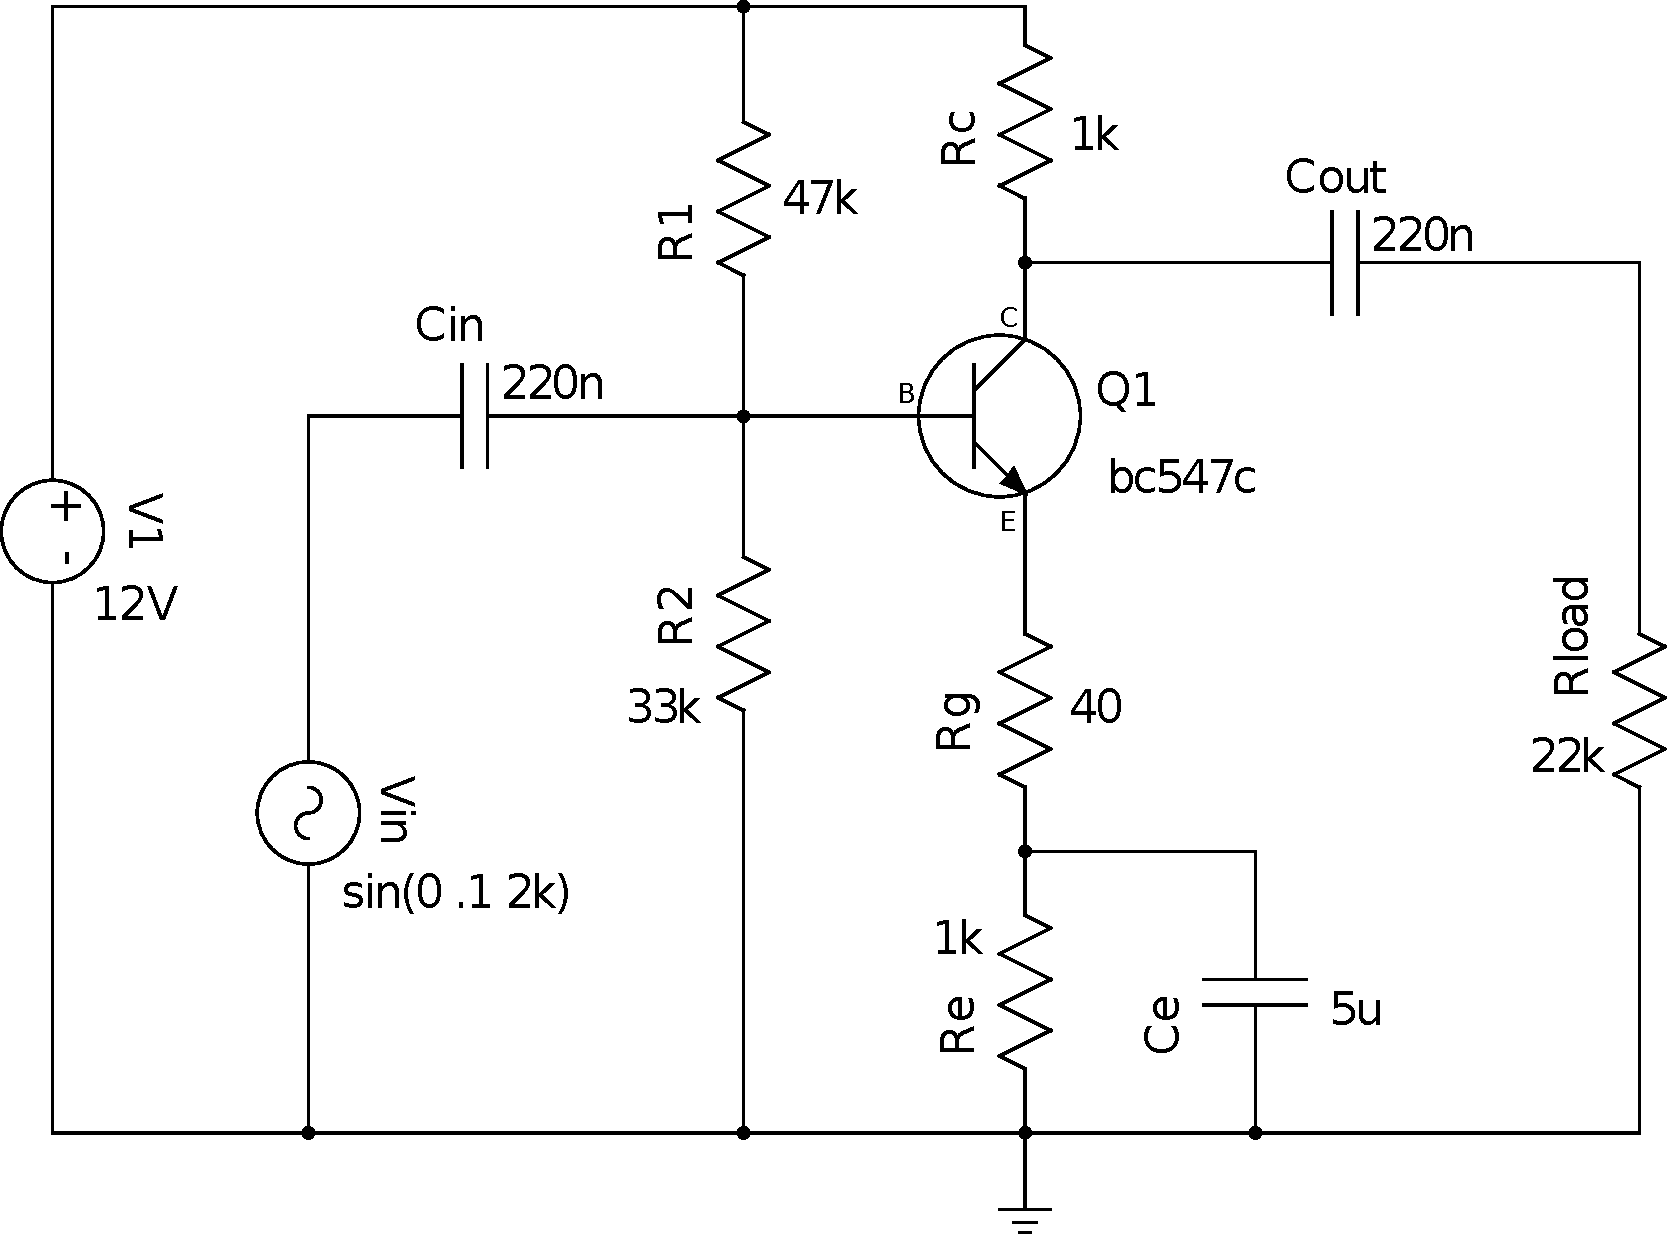
\includegraphics[scale=0.35]{ce-amplifier-simplified}
\end{frame}

\begin{frame}{Analog amplifiers}
    \centering
    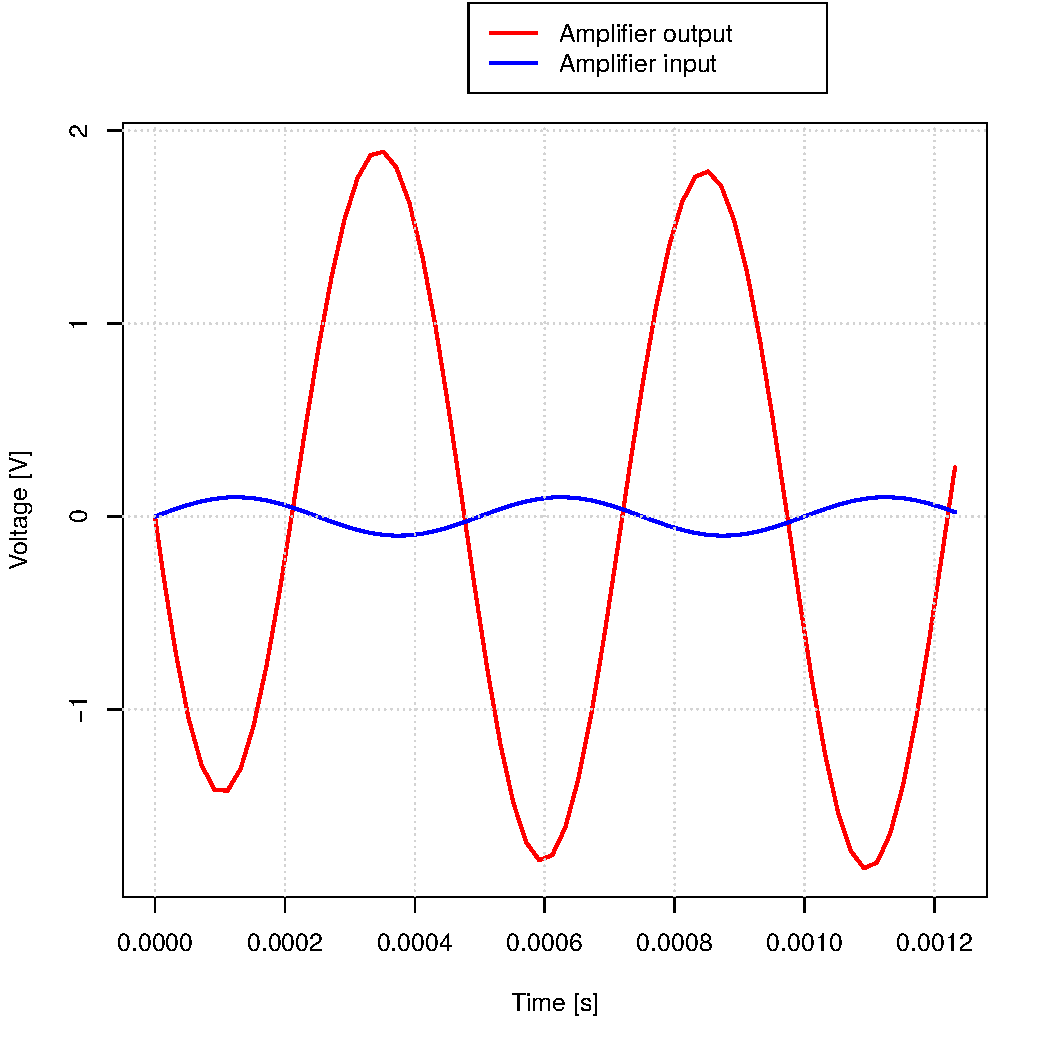
\includegraphics[scale=.45]{ce-amplifier-sim}
\end{frame}

\begin{frame}{Amplifiers evaluation}
    \centering
    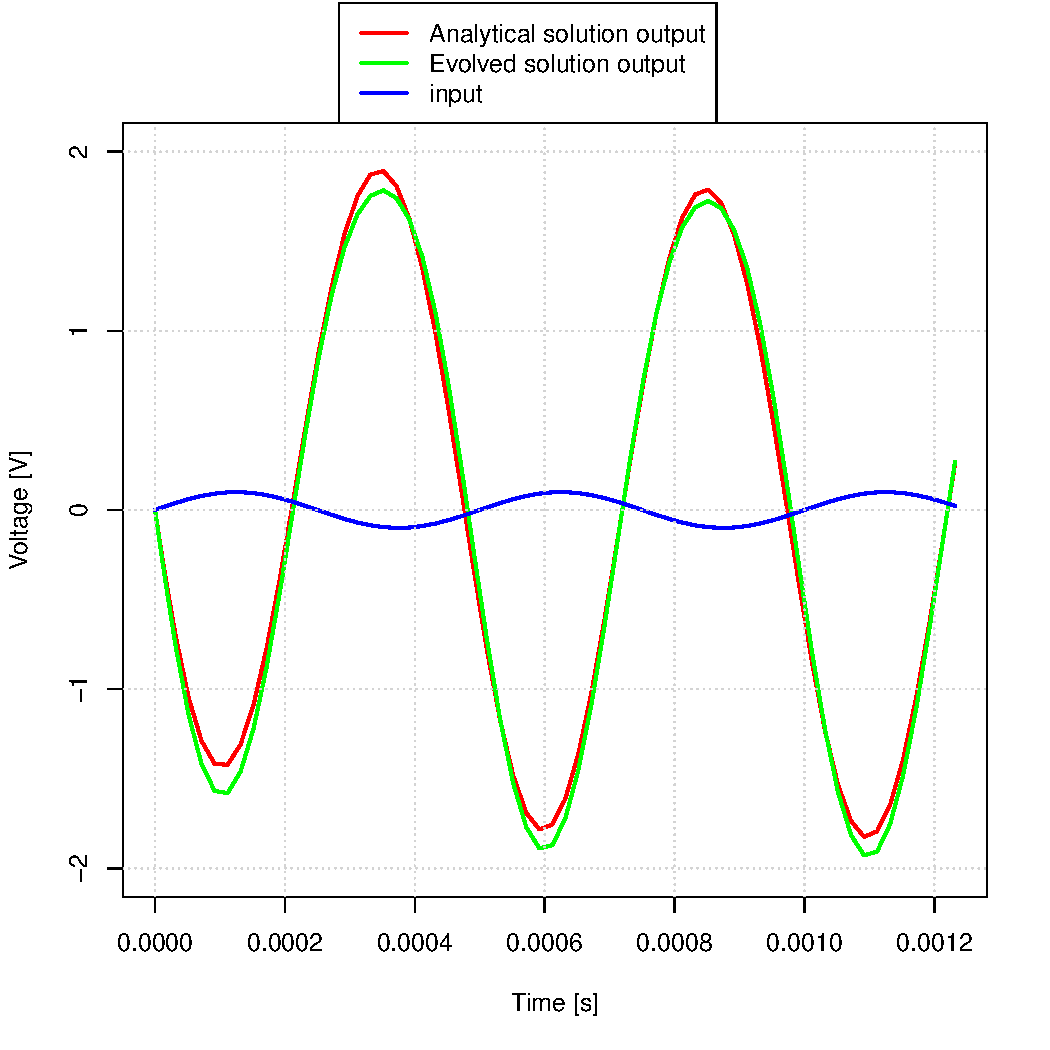
\includegraphics[scale=.45]{best-match}
\end{frame}

\begin{frame}{Amplifiers evaluation}
    \centering
    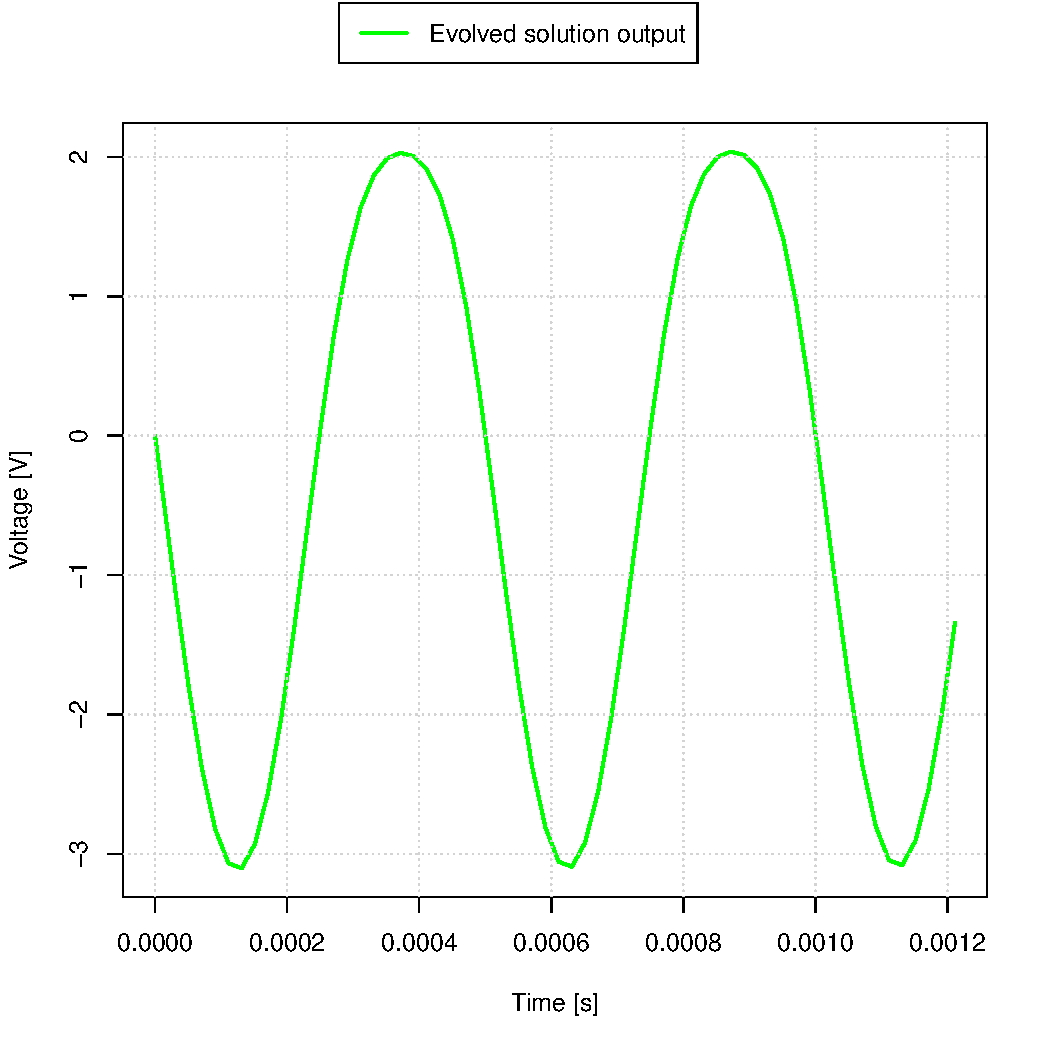
\includegraphics[scale=.45]{asymmetrical-ideal-sine}
\end{frame}

\begin{frame}{Amplifiers evaluation}
    \centering
    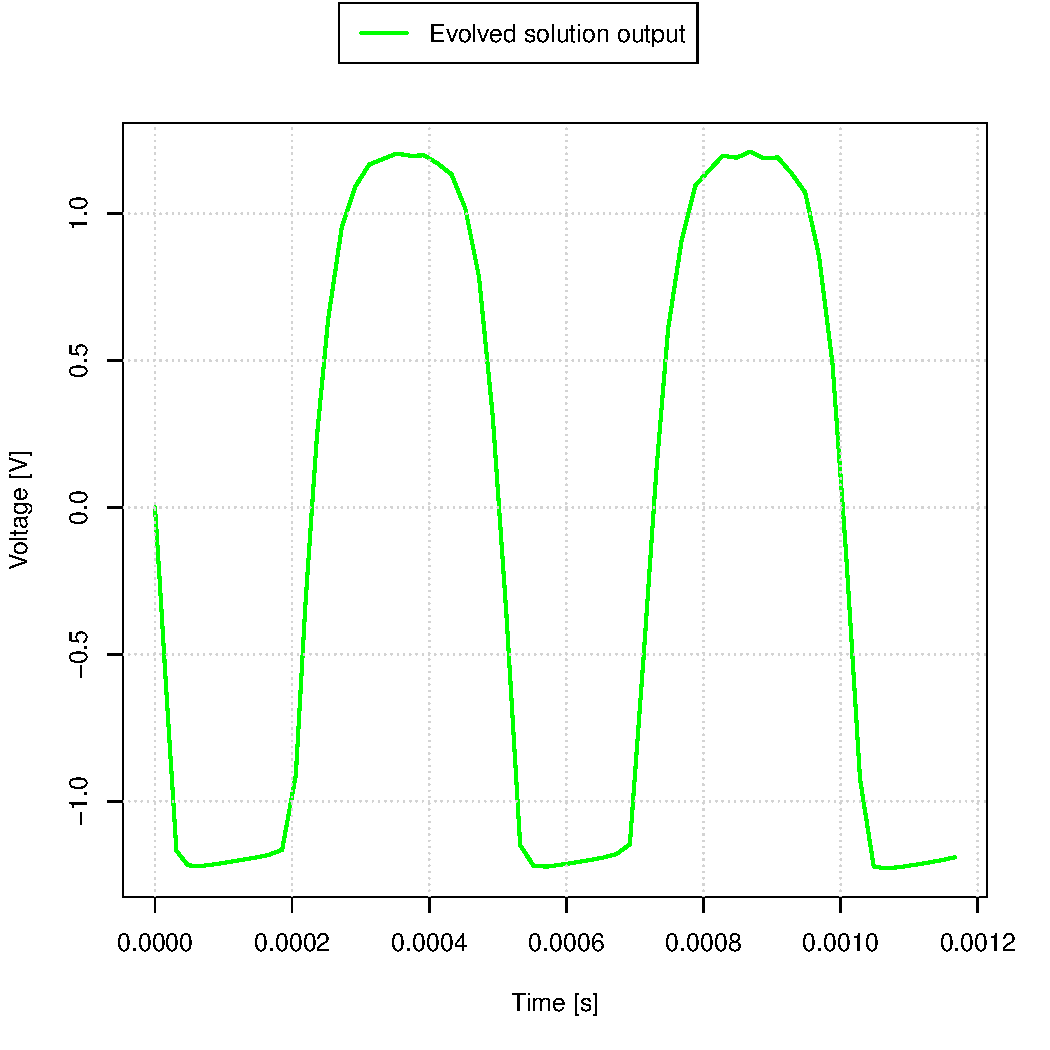
\includegraphics[scale=.4]{symmetrical-ideal-sine}

    \[
        result = (|peak + trough| + 1) \cdot fitness
    \]
\end{frame}

\begin{frame}{Experiments}

\centering
{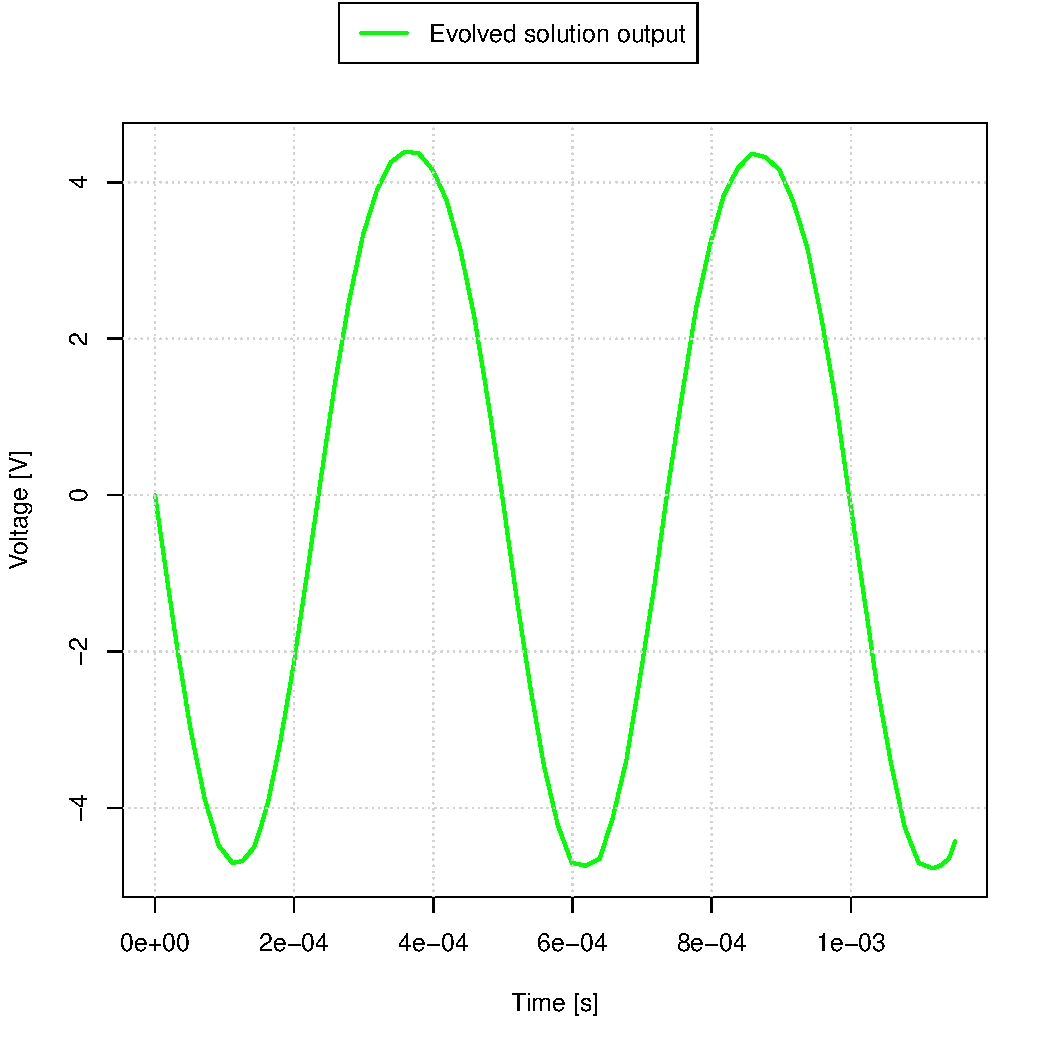
\includegraphics[scale=0.35]{best-solution-single-stage}}

\begin{table}[H]
\begin{adjustbox}{max width=\textwidth}
\begin{tabular}{@{}cccccccc@{}}
\toprule
    $R1$ [\si{\kilo\ohm}] & $R2$ [\si{\kilo\ohm}] & $Re$ [\si{\ohm}] & $Rg$ [\si{\ohm}] & $Rc$ [\si{\kilo\ohm}] & $Ce$ [\si{\micro\farad}] & $Cin$ [\si{\micro\farad}] & $Cout$ [\si{\nano\farad}] \\
    \midrule
    168 & 15.1 & 169 & 49 & 4.21 & 16 & 274 & 86 \\
    \bottomrule
\end{tabular}
\end{adjustbox}
\end{table}
\end{frame}

\begin{frame}\frametitle{Results}
    \begin{itemize}
        \item A demonstration of evolution strategies. \newline
        \item Contribution to the ngSPICE project:
            \begin{itemize}
                \item \textit{‘Hello Marek,\\
                        Thank you for this patch. It is a good pointer to some places.\\
                        ...,\\
                        we will see where it fits best.\\
                        Thank You.’ \newline}
                        Robert Larice \newline
            \end{itemize}
        \item A tool for designing analog amplifiers.
        \
    \end{itemize}
\end{frame}

\begin{frame}{Evolution example} \centering 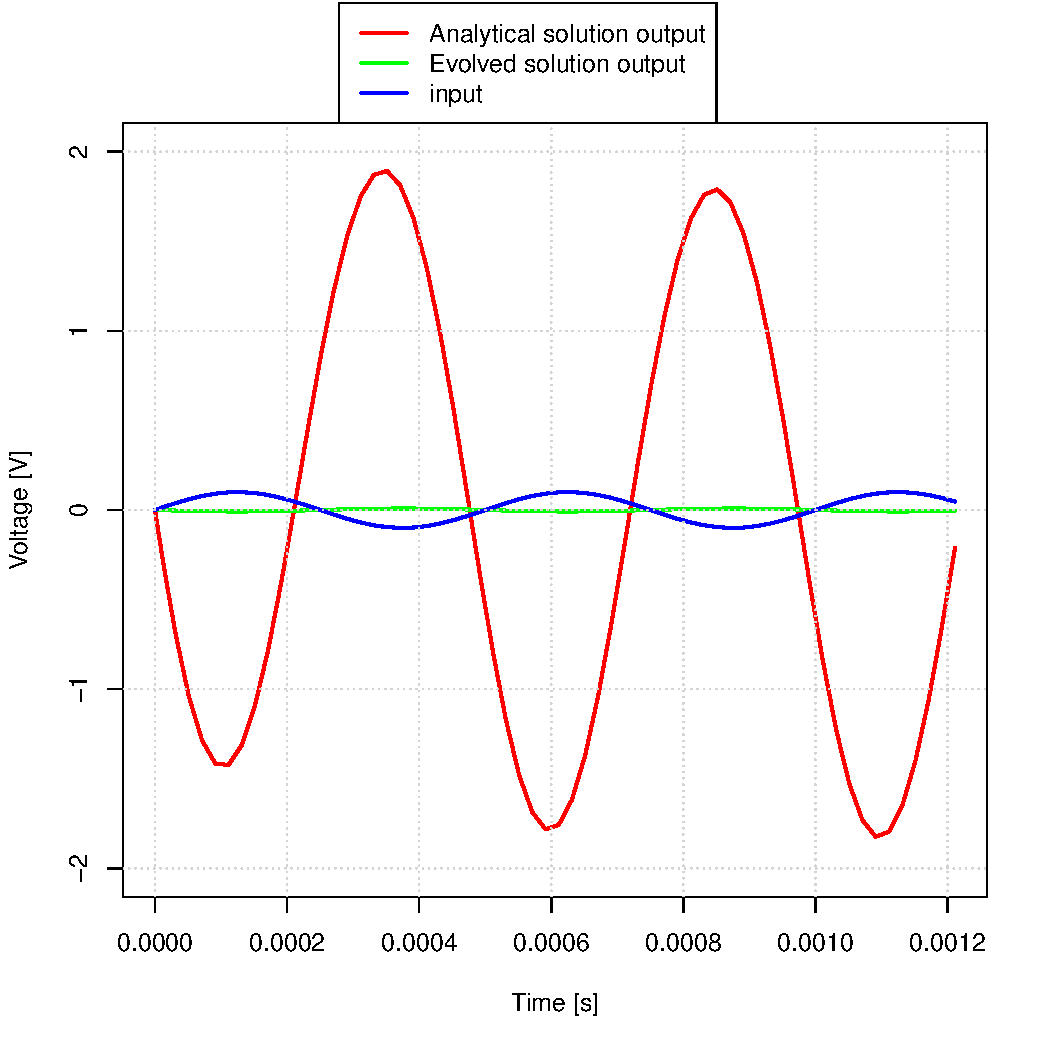
\includegraphics[scale=0.45]{evolutionCourse/graph00} \end{frame}
\begin{frame}{Evolution example} \centering 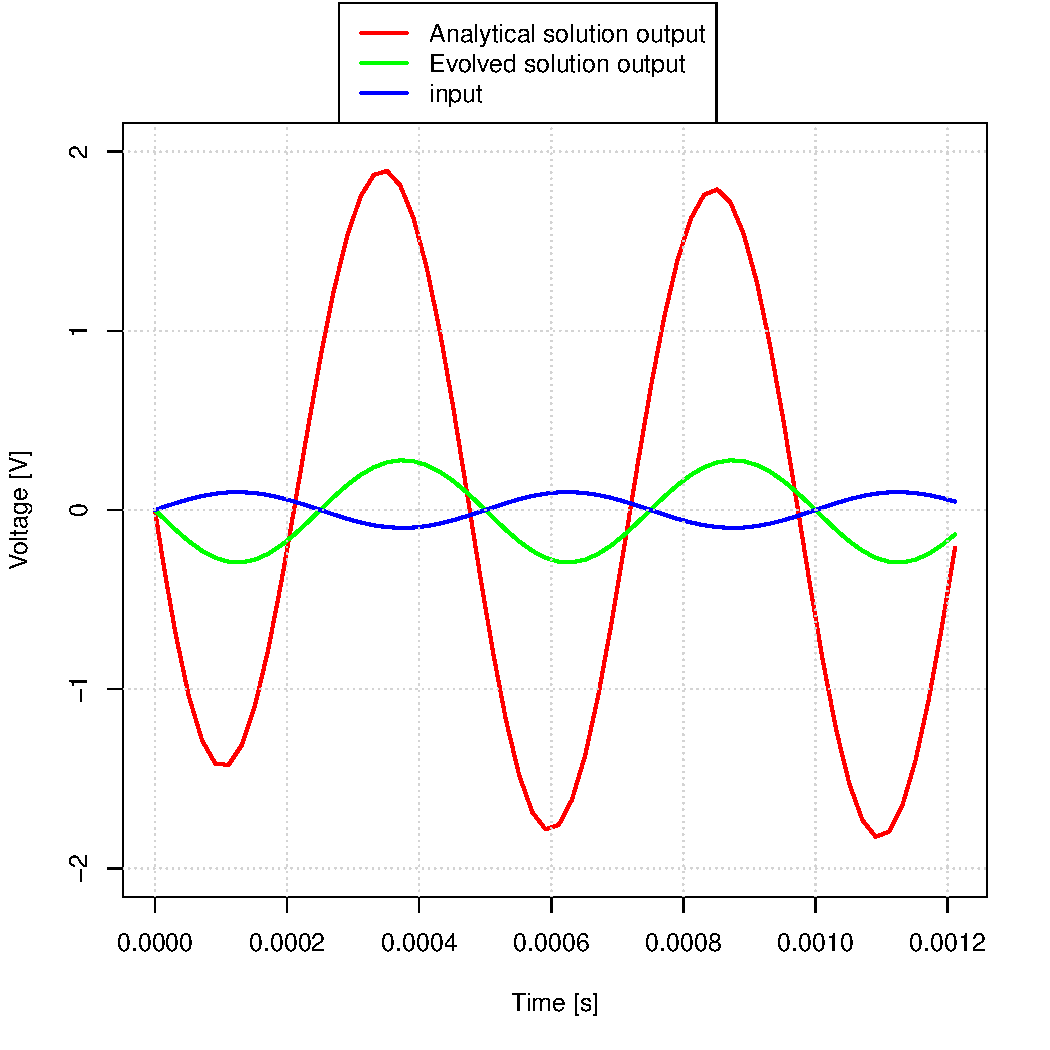
\includegraphics[scale=0.45]{evolutionCourse/graph01} \end{frame}
\begin{frame}{Evolution example} \centering 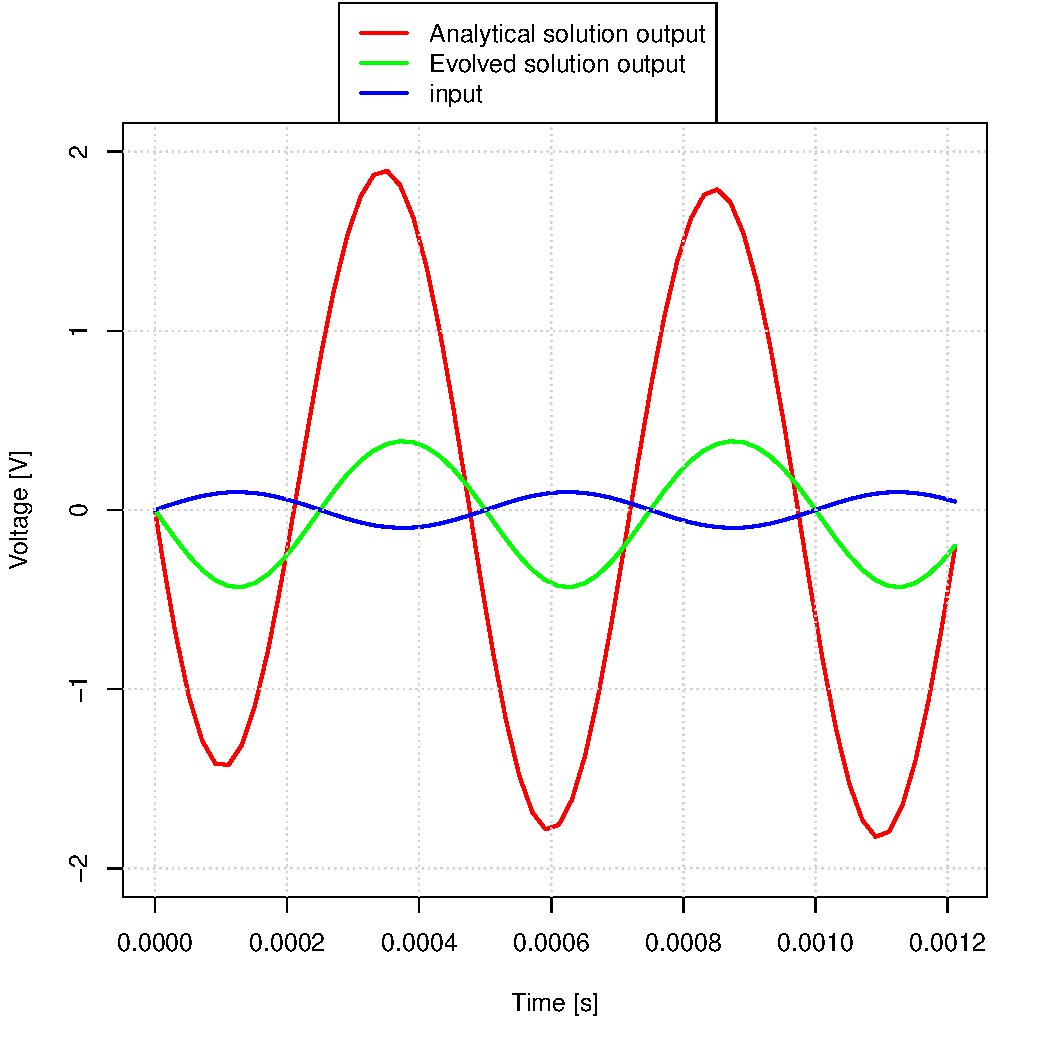
\includegraphics[scale=0.45]{evolutionCourse/graph02} \end{frame}
\begin{frame}{Evolution example} \centering 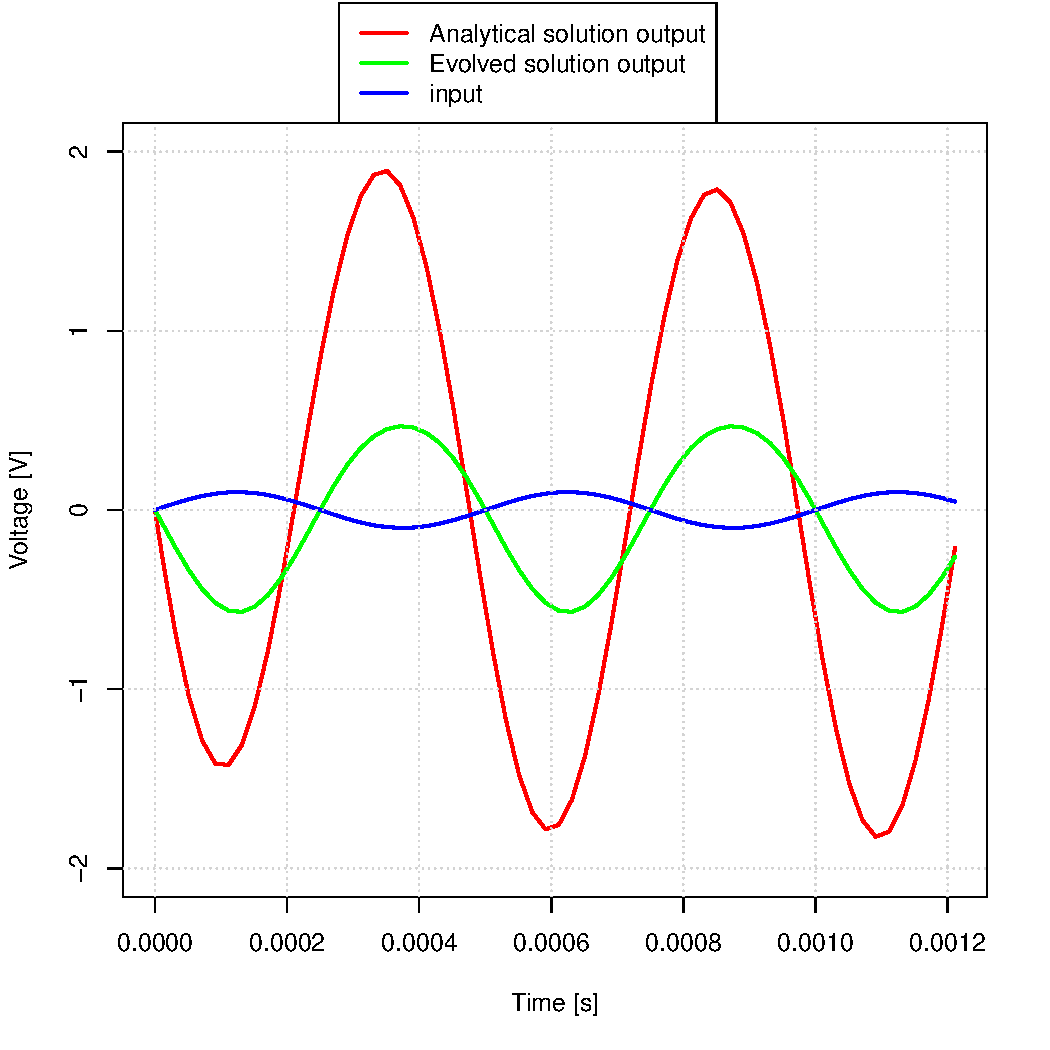
\includegraphics[scale=0.45]{evolutionCourse/graph03} \end{frame}
\begin{frame}{Evolution example} \centering 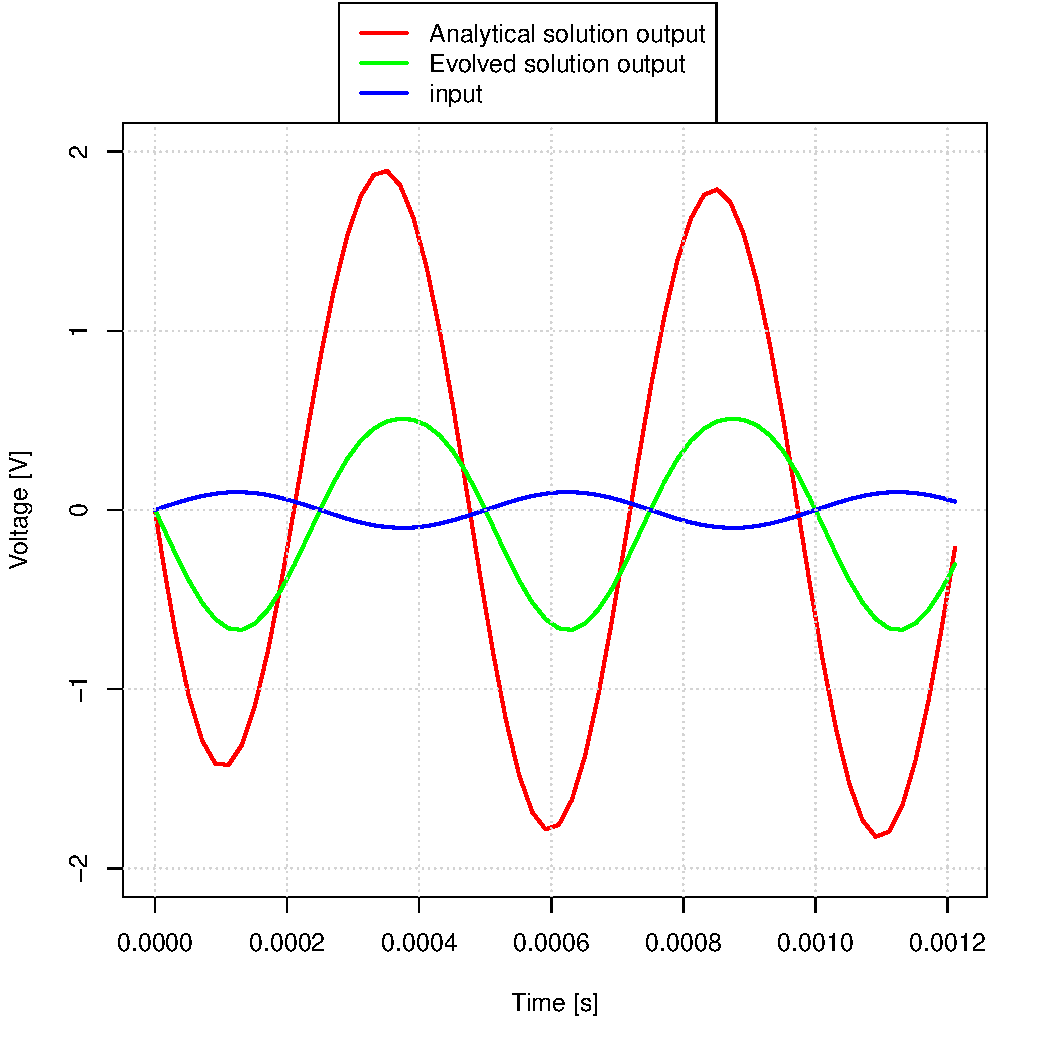
\includegraphics[scale=0.45]{evolutionCourse/graph04} \end{frame}
\begin{frame}{Evolution example} \centering 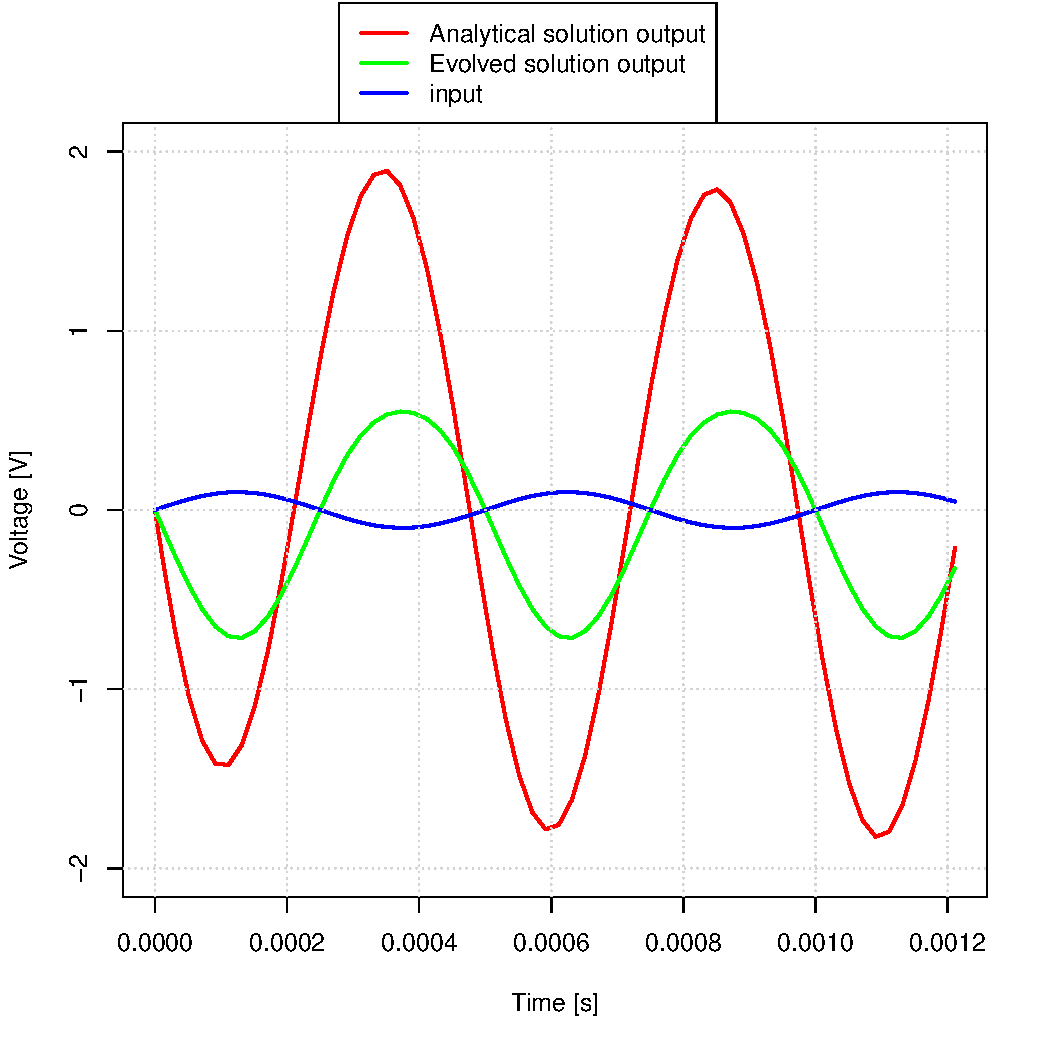
\includegraphics[scale=0.45]{evolutionCourse/graph05} \end{frame}
\begin{frame}{Evolution example} \centering 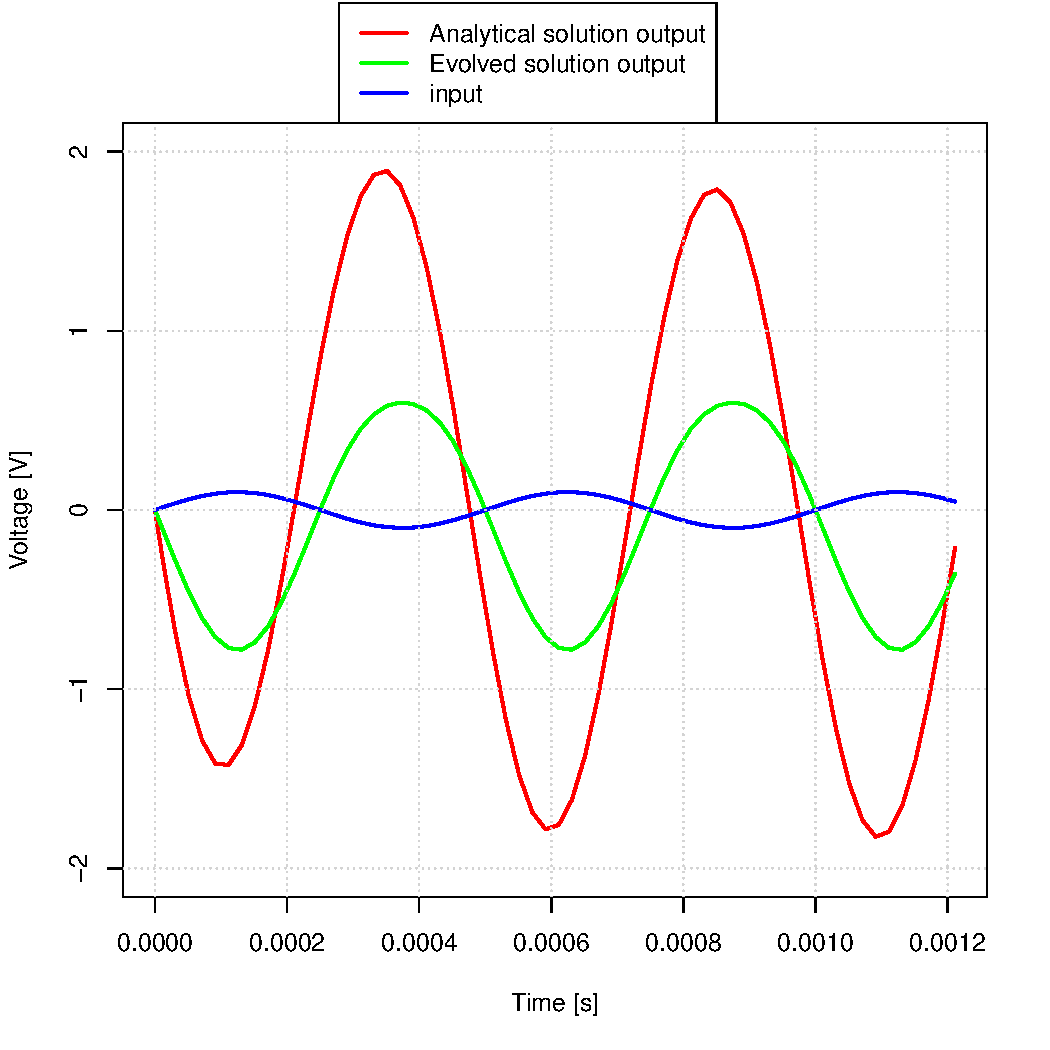
\includegraphics[scale=0.45]{evolutionCourse/graph06} \end{frame}
\begin{frame}{Evolution example} \centering 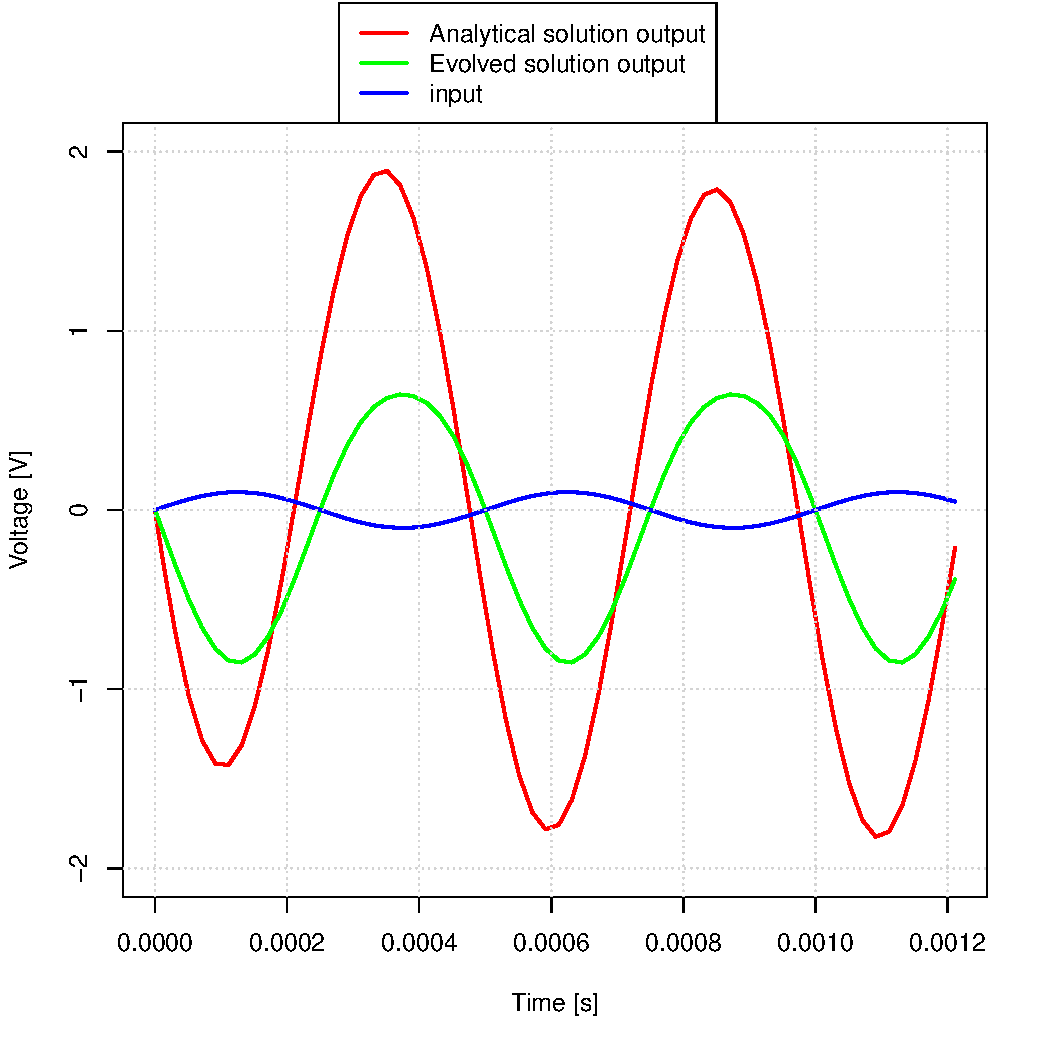
\includegraphics[scale=0.45]{evolutionCourse/graph07} \end{frame}
\begin{frame}{Evolution example} \centering 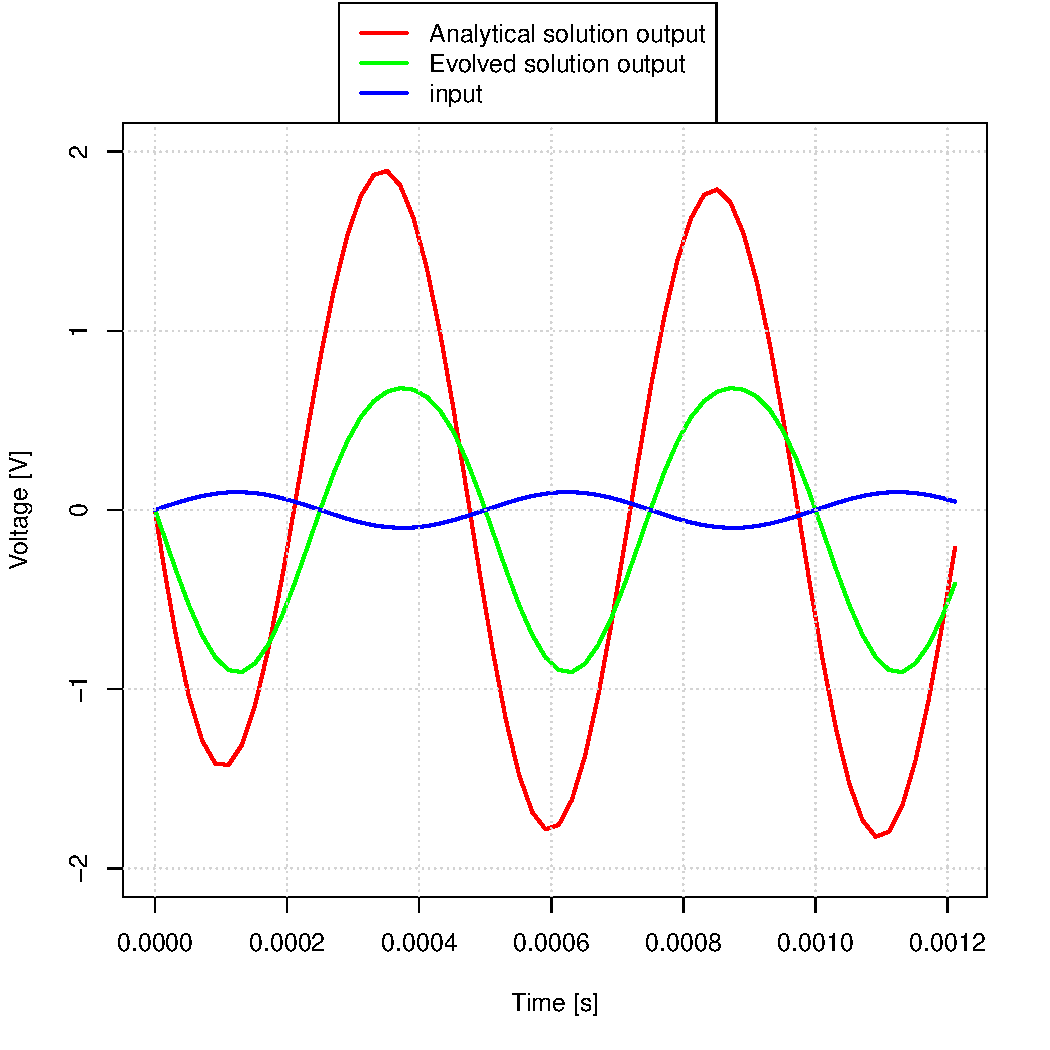
\includegraphics[scale=0.45]{evolutionCourse/graph08} \end{frame}
\begin{frame}{Evolution example} \centering 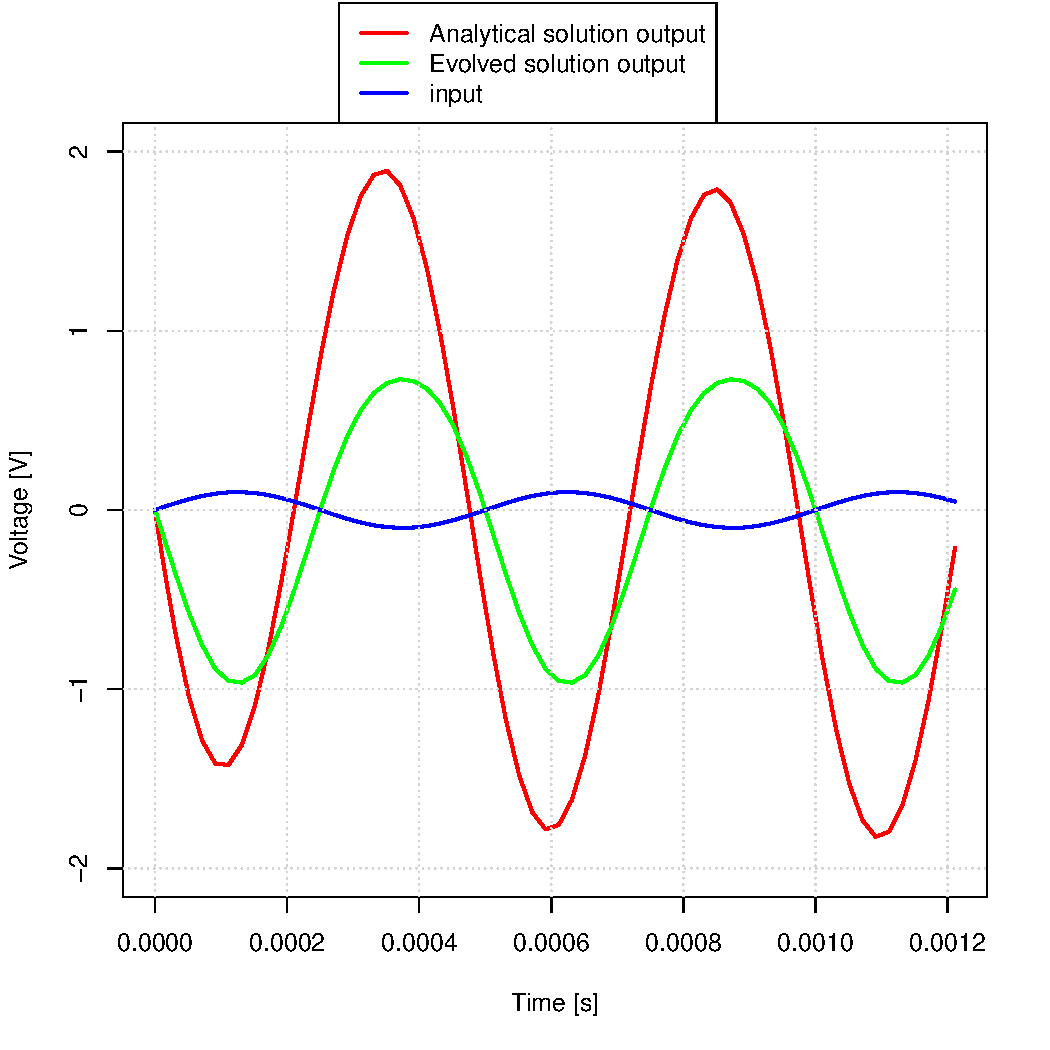
\includegraphics[scale=0.45]{evolutionCourse/graph09} \end{frame}
\begin{frame}{Evolution example} \centering 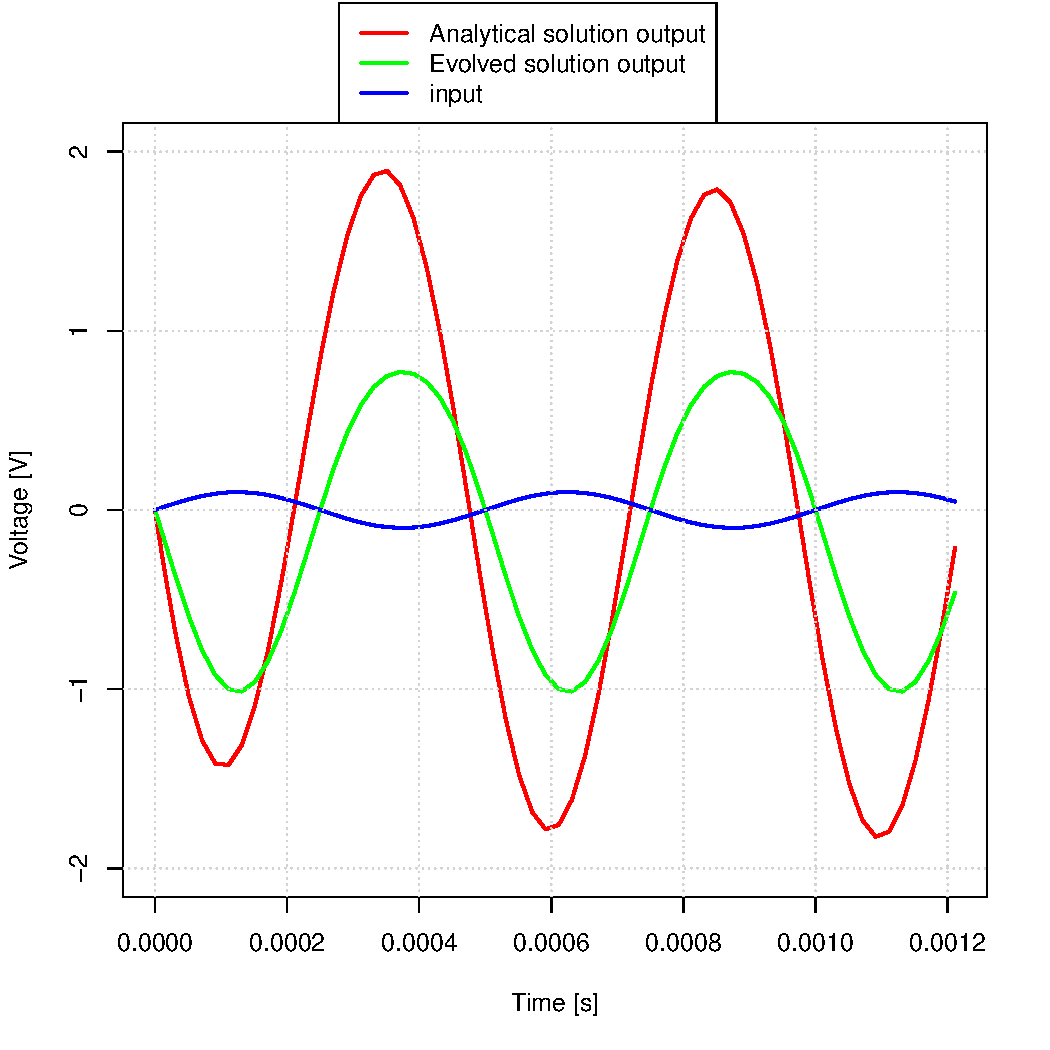
\includegraphics[scale=0.45]{evolutionCourse/graph10} \end{frame}
\begin{frame}{Evolution example} \centering 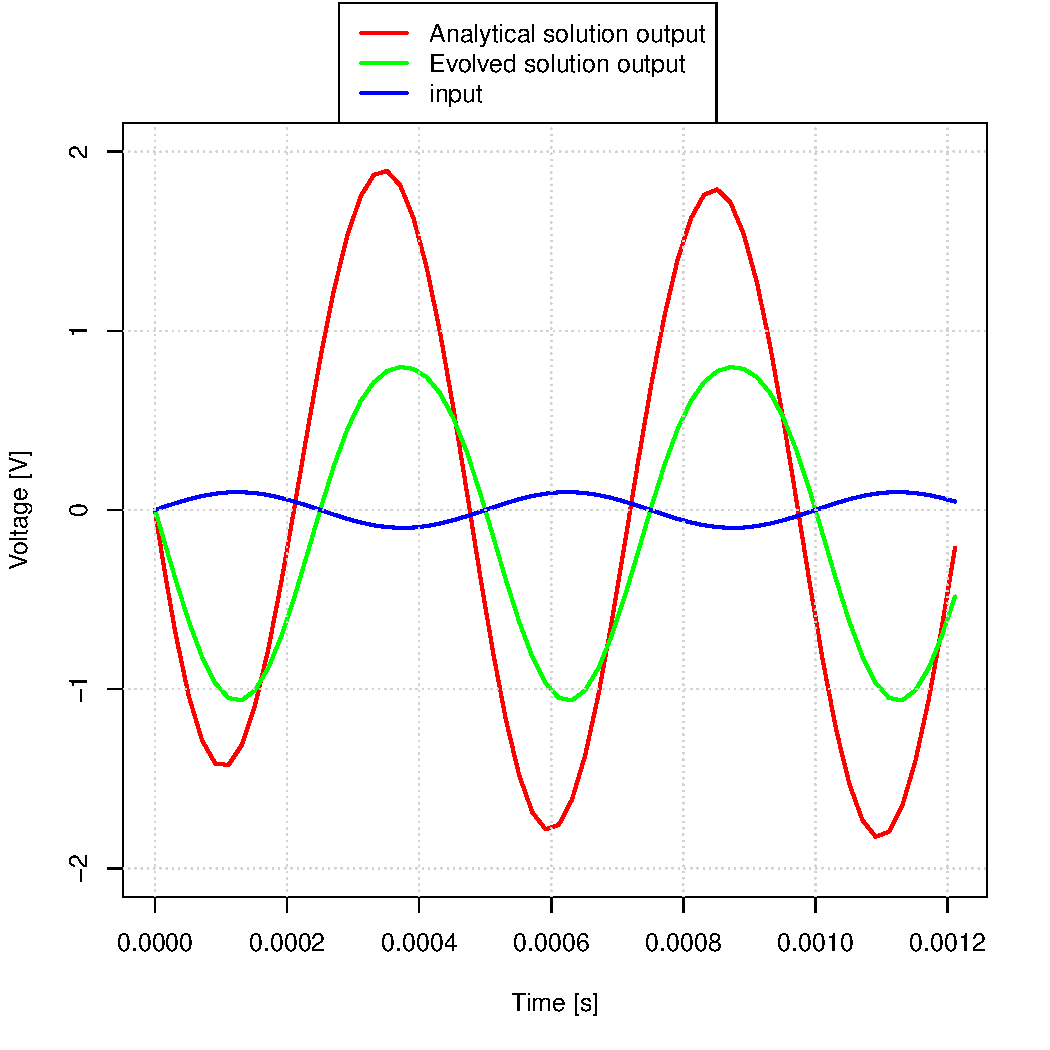
\includegraphics[scale=0.45]{evolutionCourse/graph11} \end{frame}
\begin{frame}{Evolution example} \centering 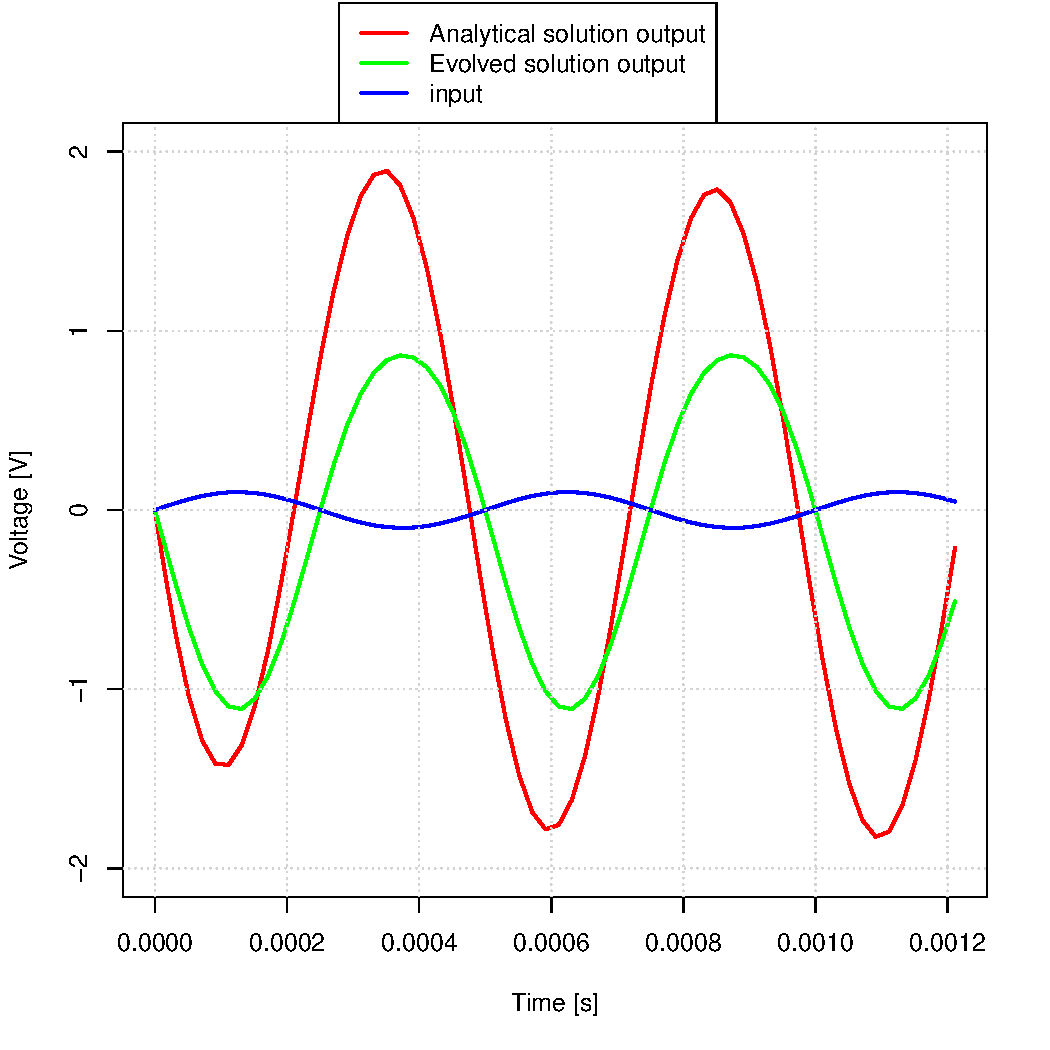
\includegraphics[scale=0.45]{evolutionCourse/graph12} \end{frame}
\begin{frame}{Evolution example} \centering 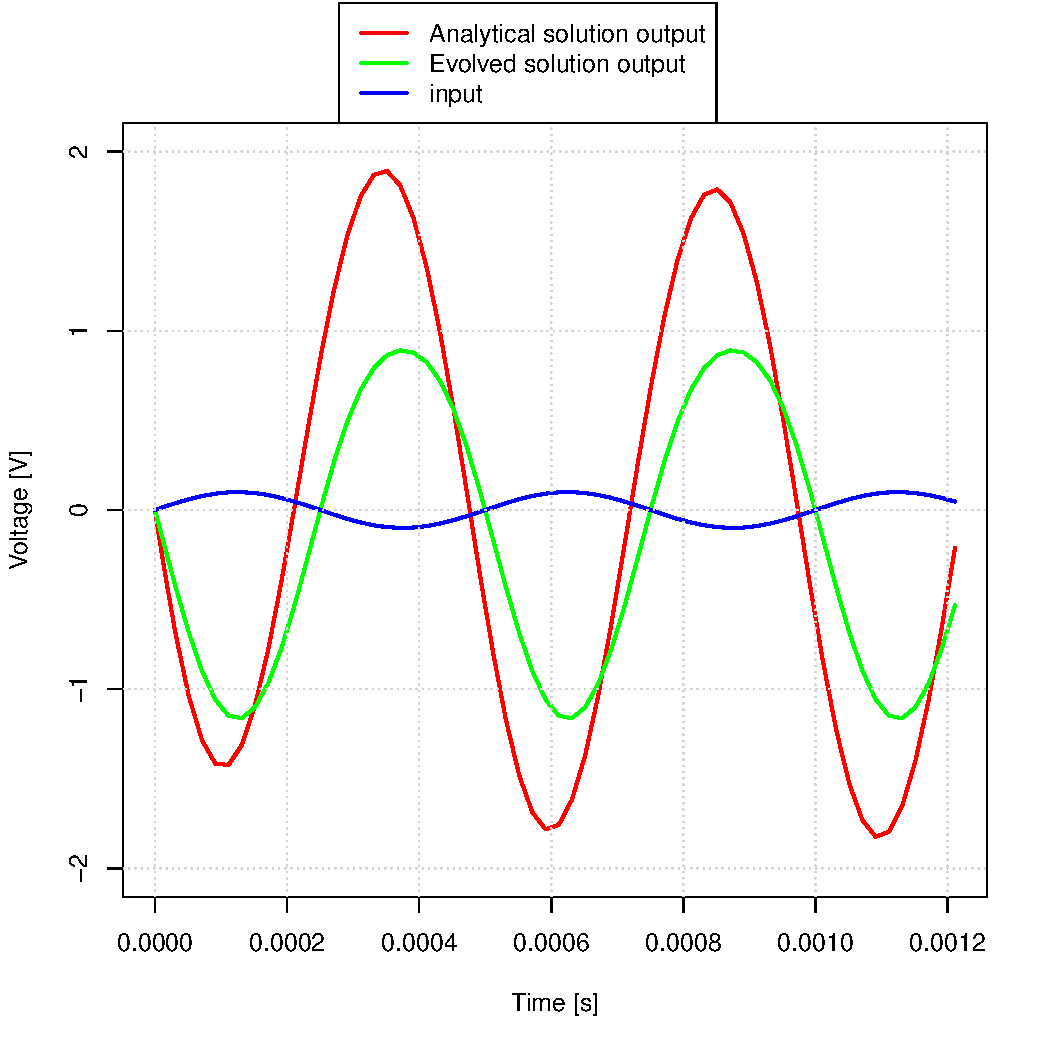
\includegraphics[scale=0.45]{evolutionCourse/graph13} \end{frame}
\begin{frame}{Evolution example} \centering 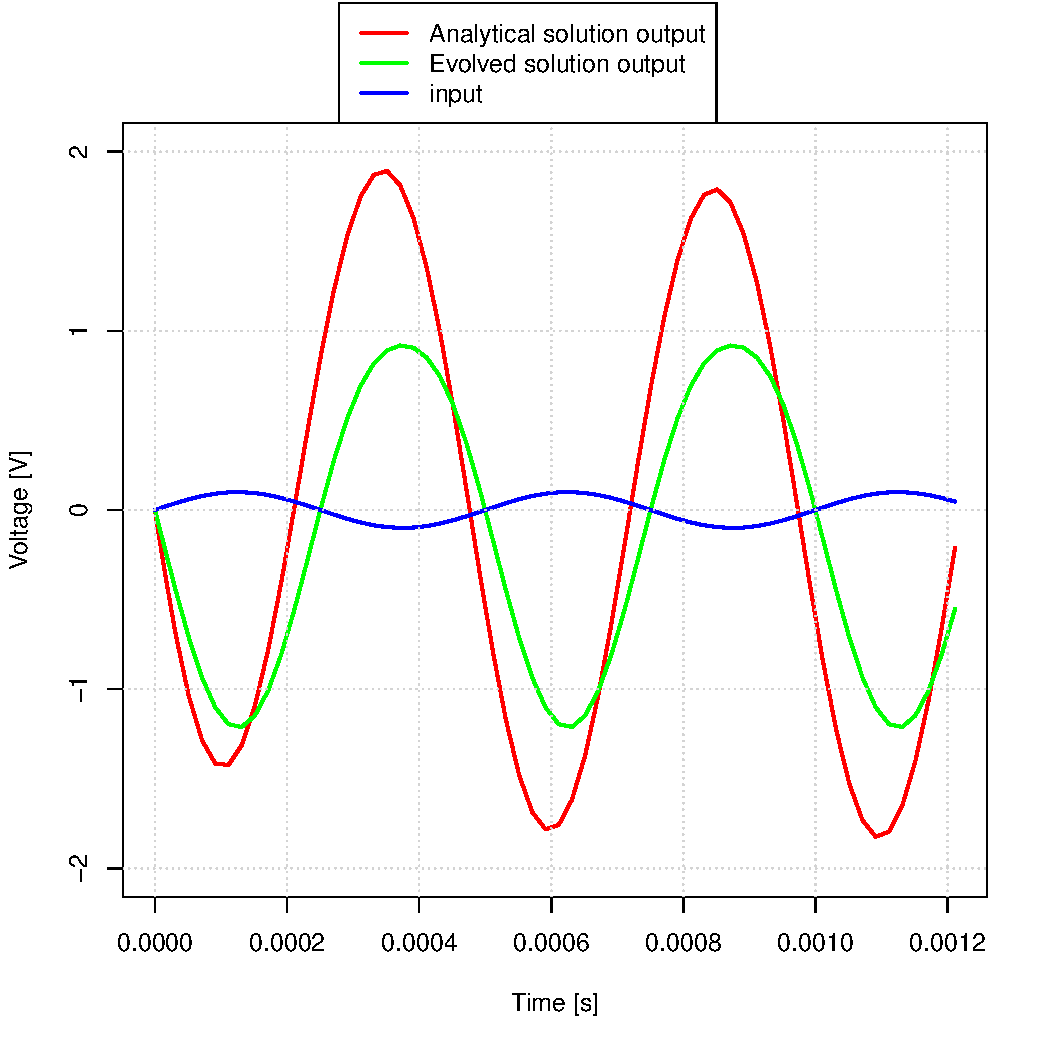
\includegraphics[scale=0.45]{evolutionCourse/graph14} \end{frame}
\begin{frame}{Evolution example} \centering 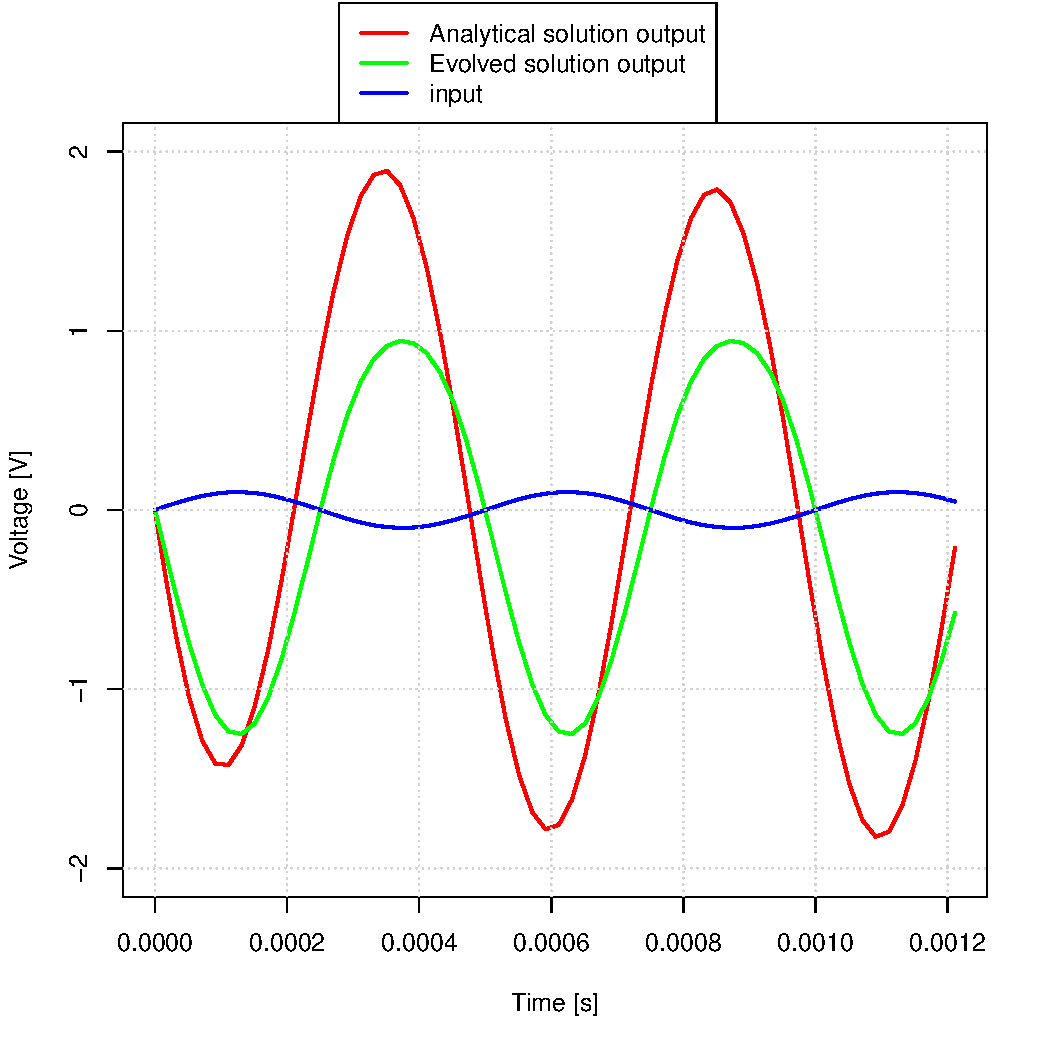
\includegraphics[scale=0.45]{evolutionCourse/graph15} \end{frame}
\begin{frame}{Evolution example} \centering 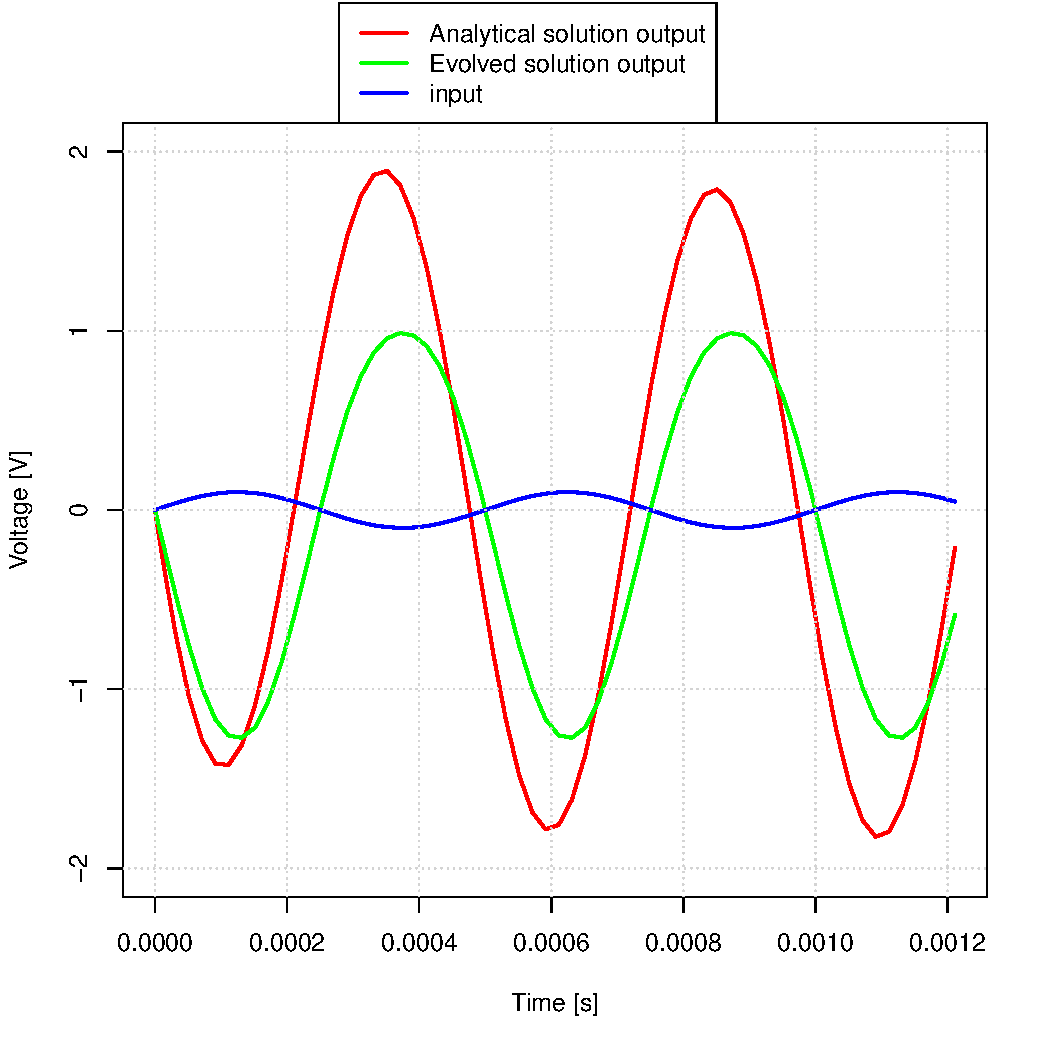
\includegraphics[scale=0.45]{evolutionCourse/graph16} \end{frame}
\begin{frame}{Evolution example} \centering 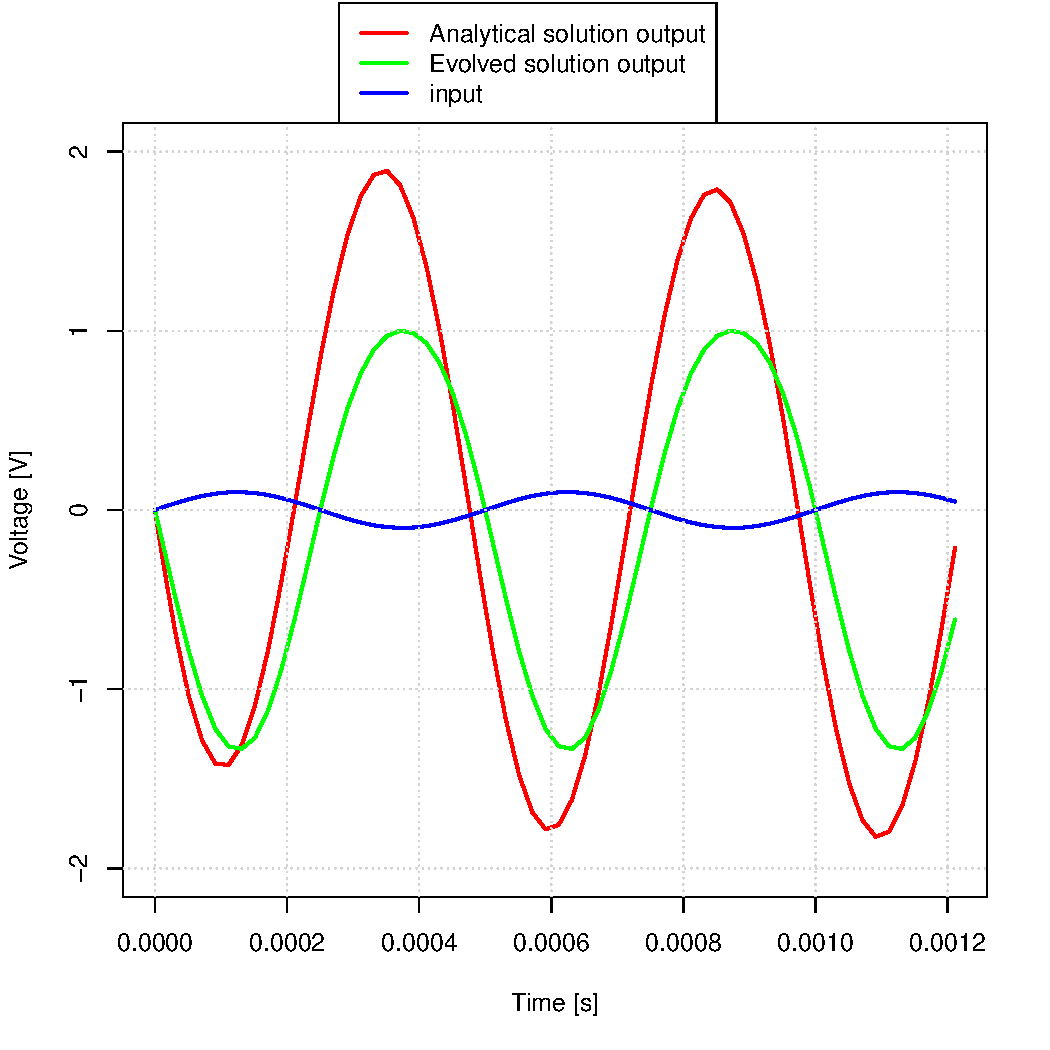
\includegraphics[scale=0.45]{evolutionCourse/graph17} \end{frame}
\begin{frame}{Evolution example} \centering 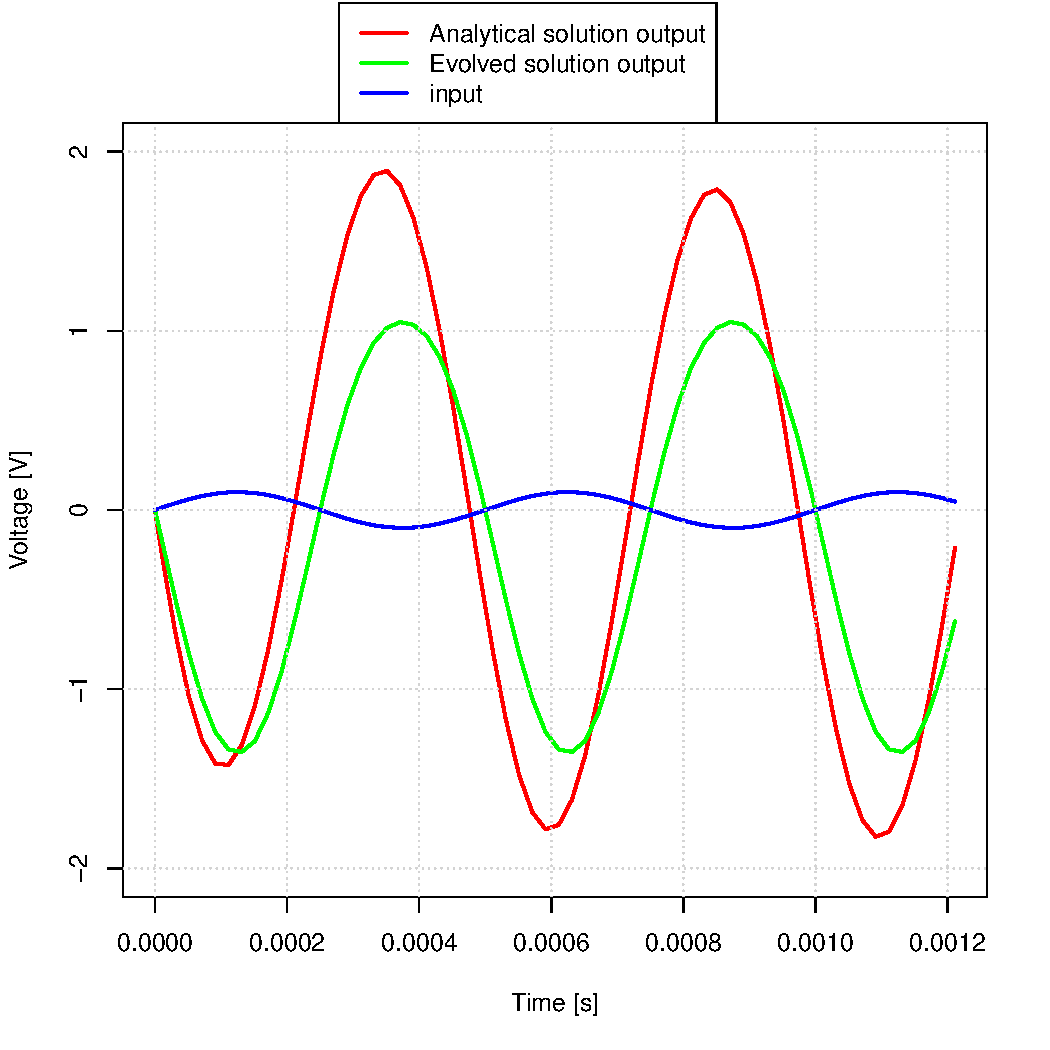
\includegraphics[scale=0.45]{evolutionCourse/graph18} \end{frame}
\begin{frame}{Evolution example} \centering 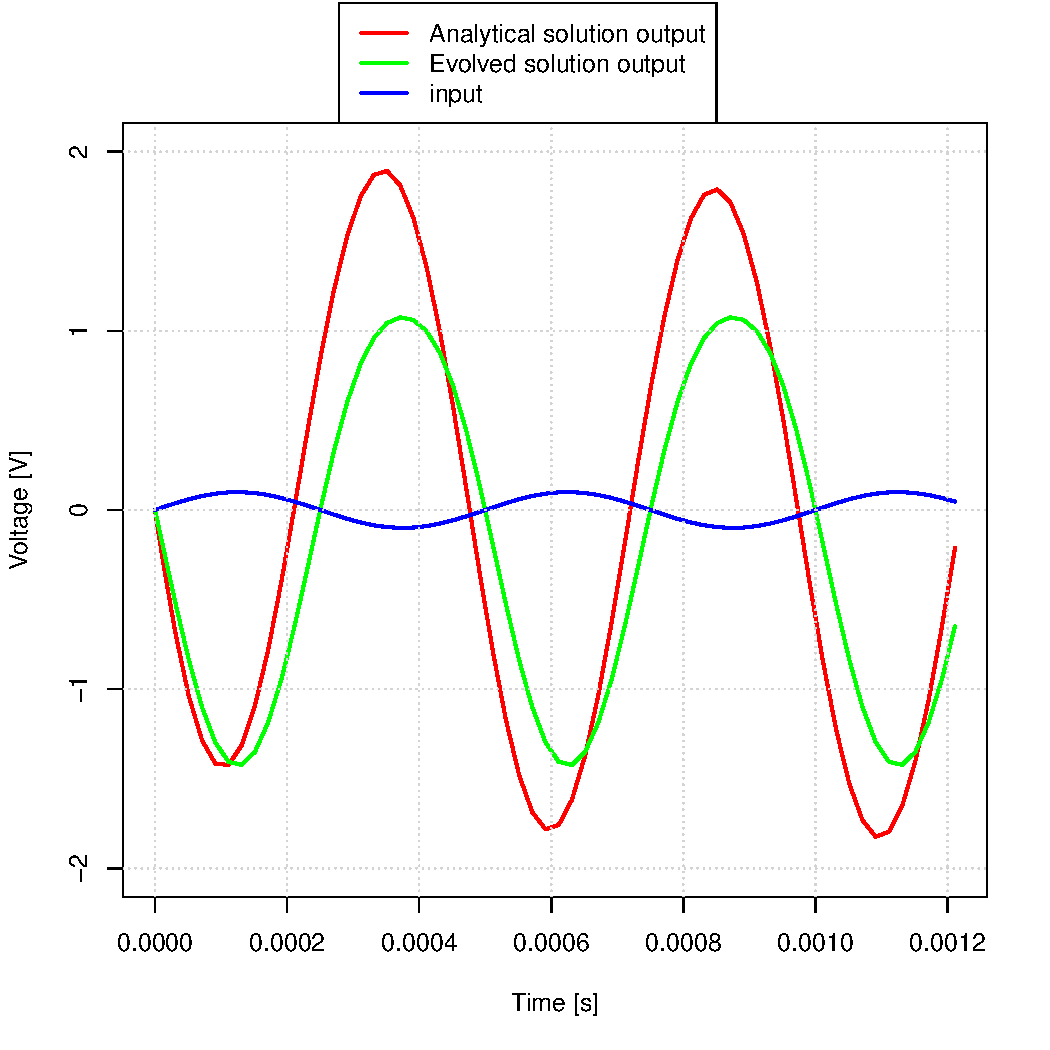
\includegraphics[scale=0.45]{evolutionCourse/graph19} \end{frame}
\begin{frame}{Evolution example} \centering 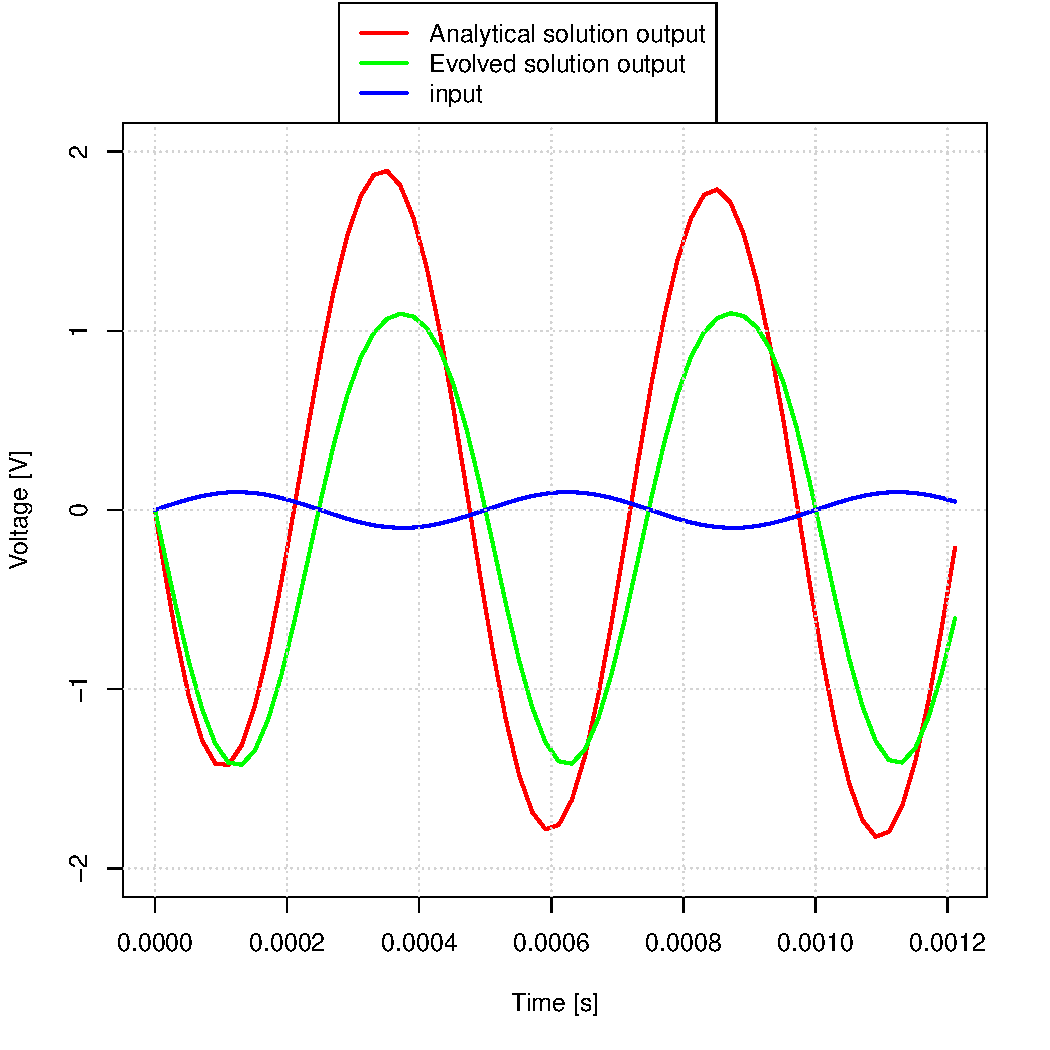
\includegraphics[scale=0.45]{evolutionCourse/graph20} \end{frame}
\begin{frame}{Evolution example} \centering 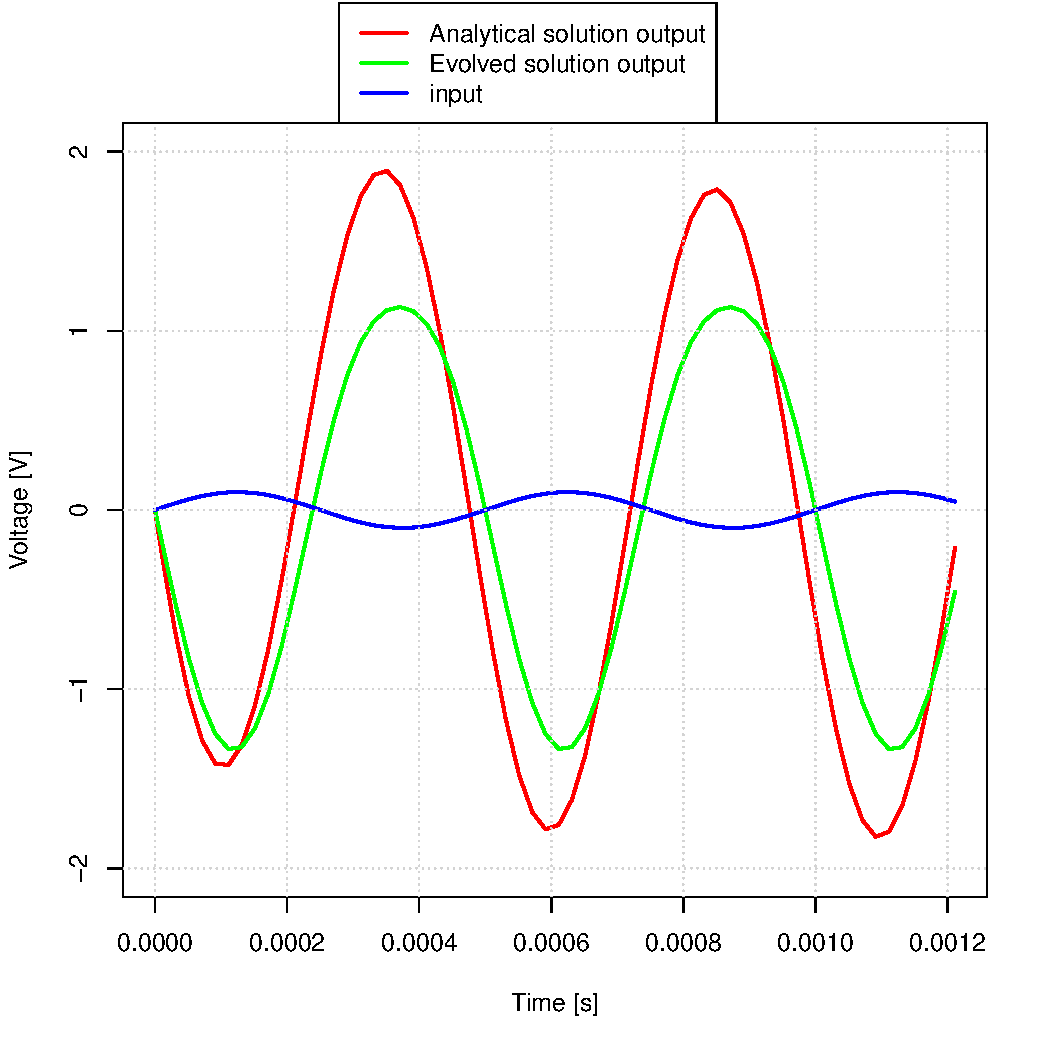
\includegraphics[scale=0.45]{evolutionCourse/graph21} \end{frame}
\begin{frame}{Evolution example} \centering 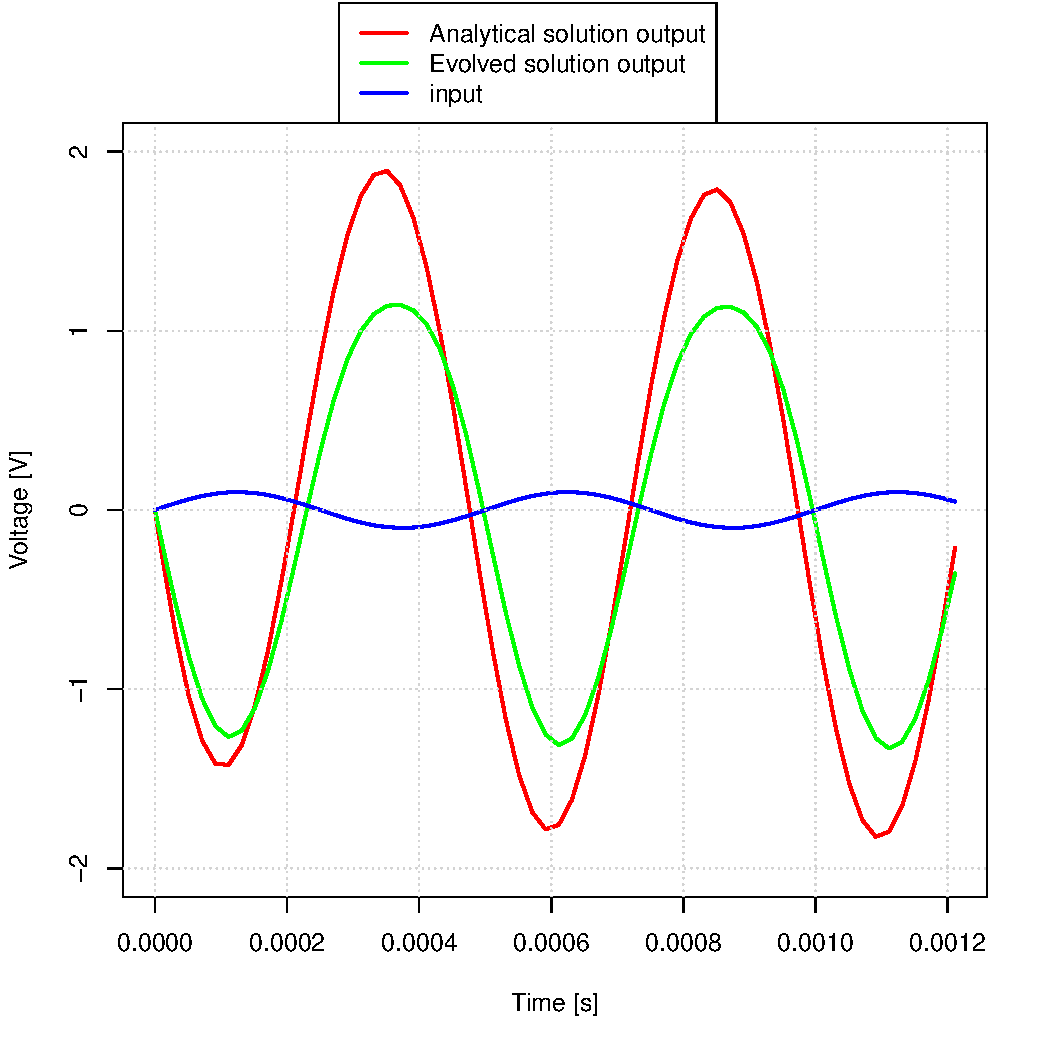
\includegraphics[scale=0.45]{evolutionCourse/graph22} \end{frame}
\begin{frame}{Evolution example} \centering 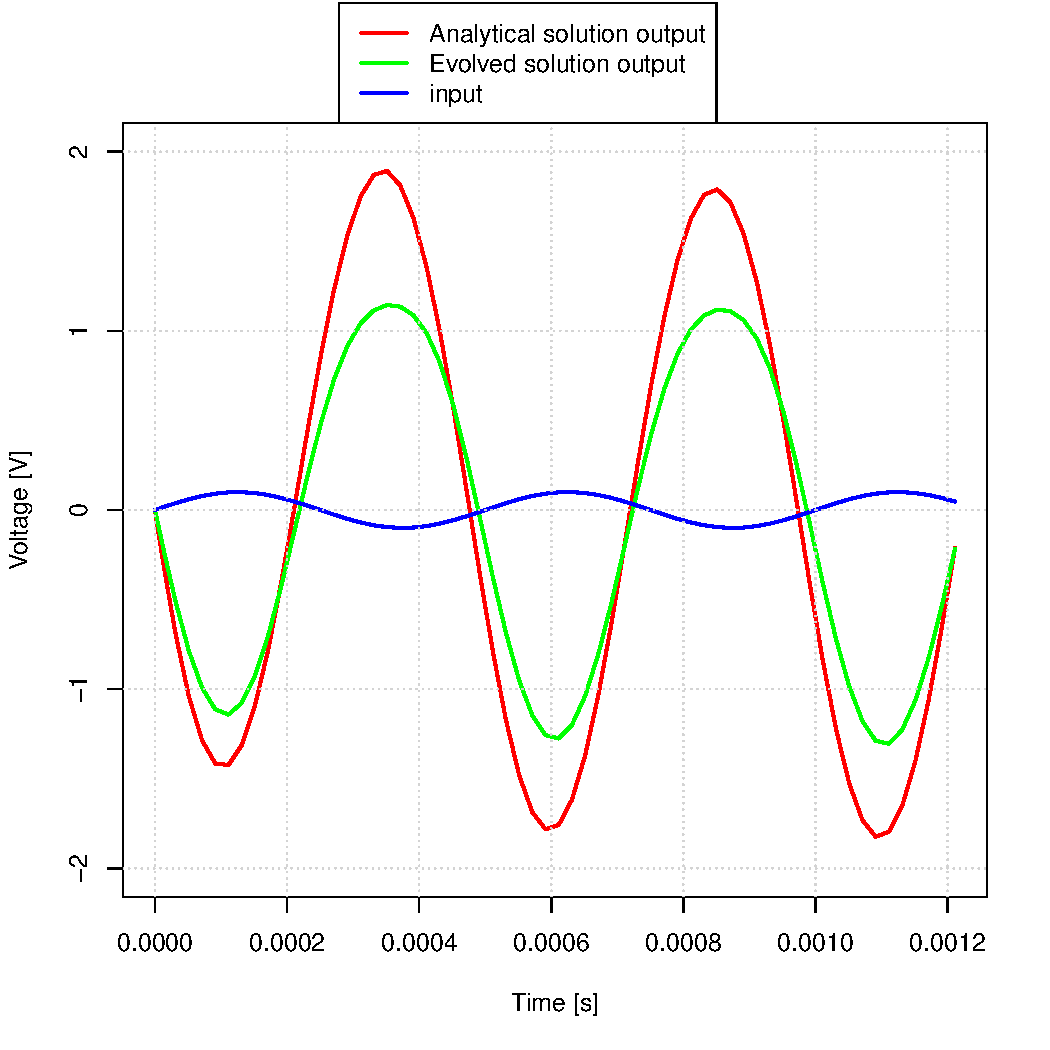
\includegraphics[scale=0.45]{evolutionCourse/graph23} \end{frame}
\begin{frame}{Evolution example} \centering 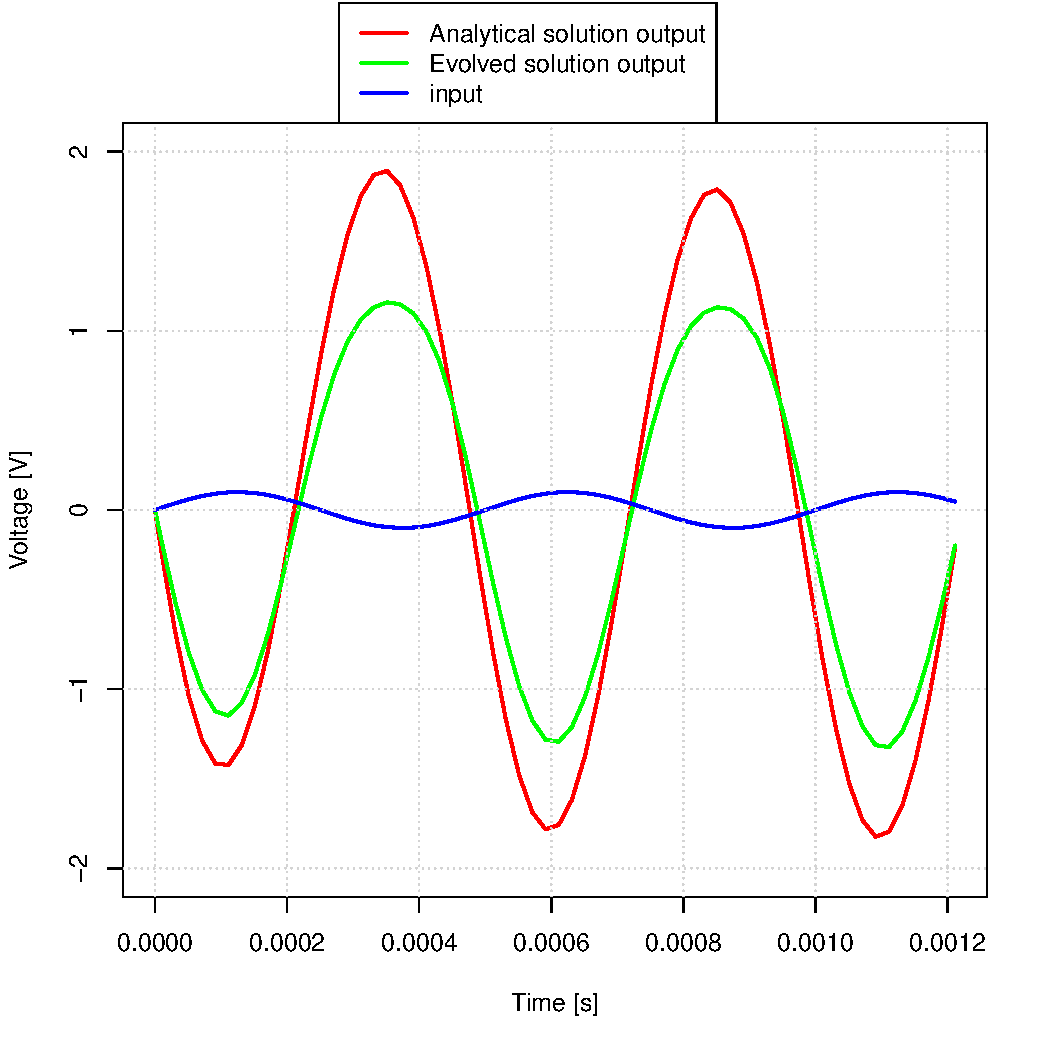
\includegraphics[scale=0.45]{evolutionCourse/graph24} \end{frame}
\begin{frame}{Evolution example} \centering 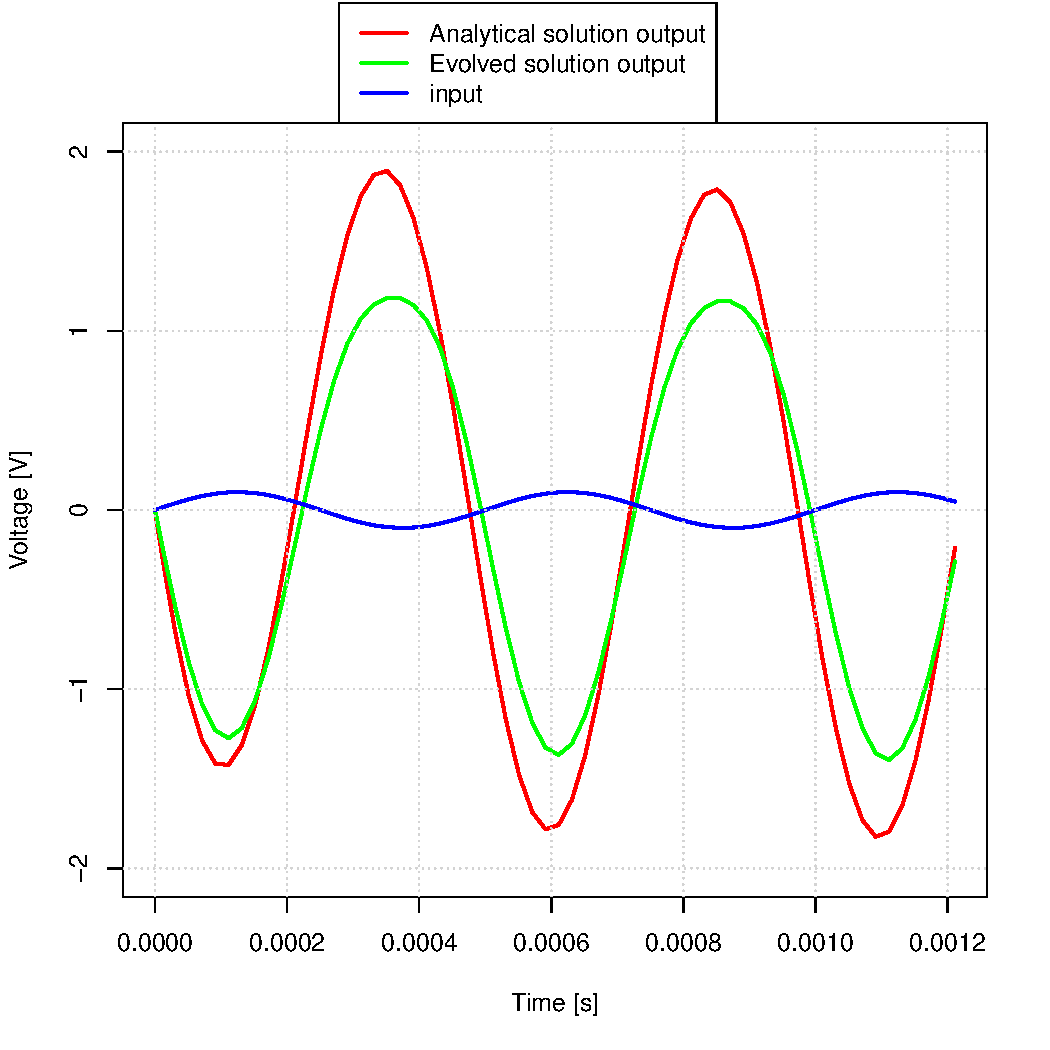
\includegraphics[scale=0.45]{evolutionCourse/graph25} \end{frame}
\begin{frame}{Evolution example} \centering 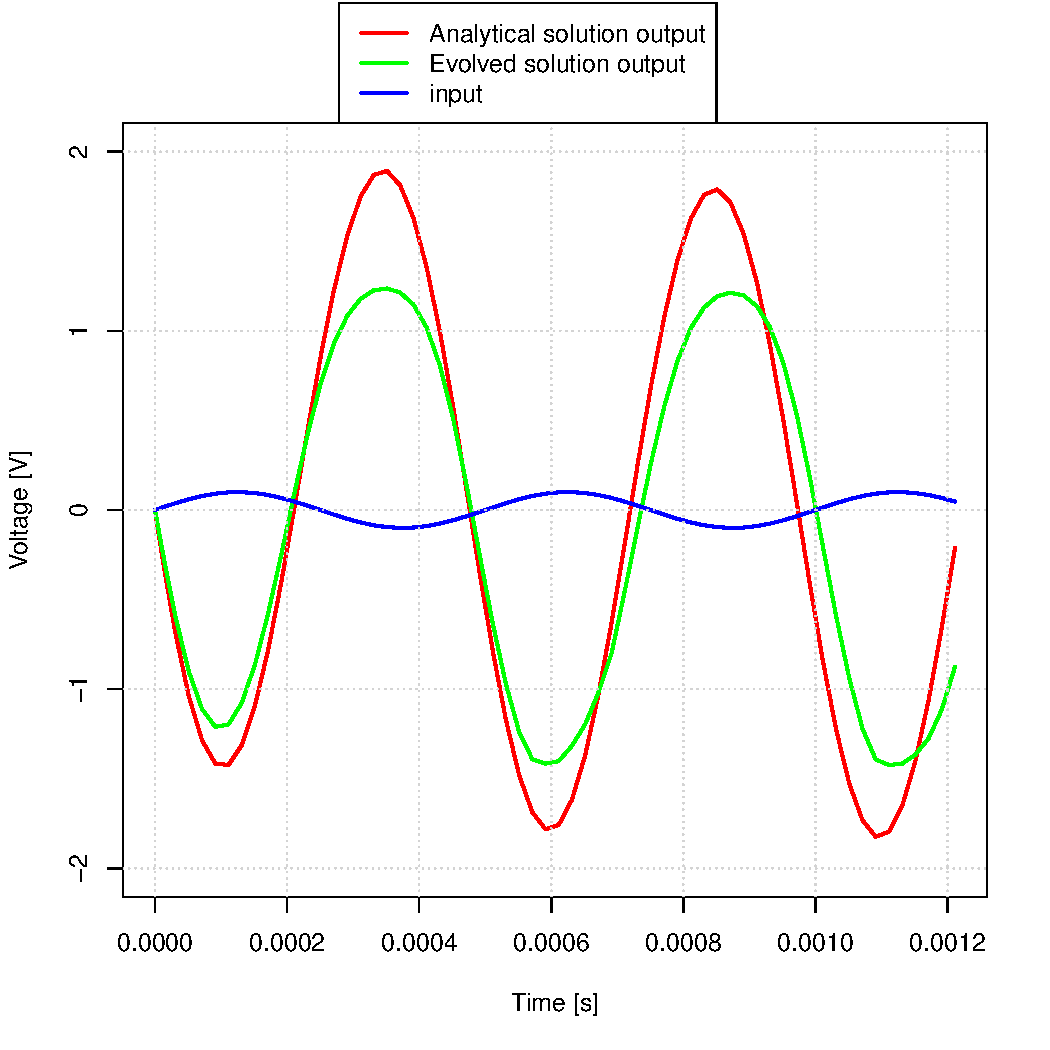
\includegraphics[scale=0.45]{evolutionCourse/graph26} \end{frame}
\begin{frame}{Evolution example} \centering 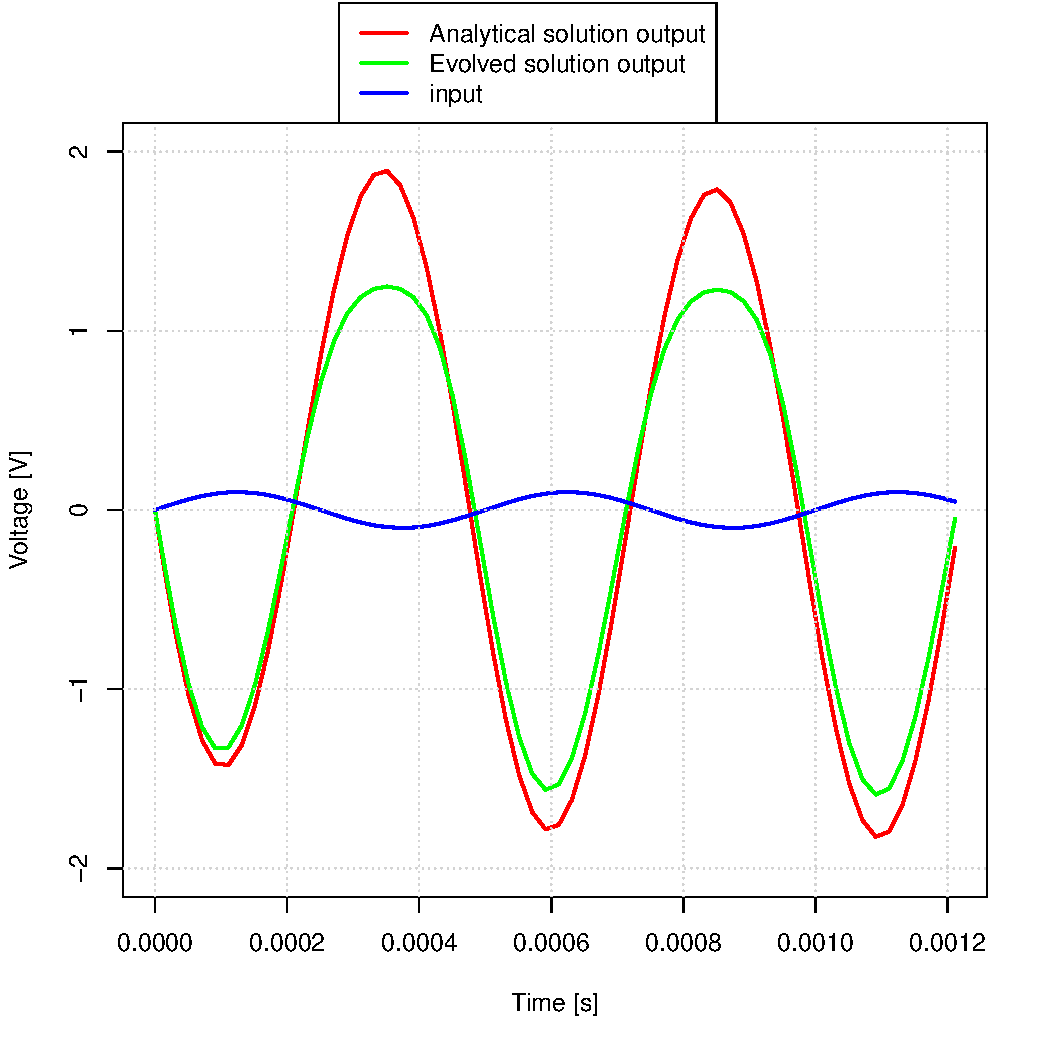
\includegraphics[scale=0.45]{evolutionCourse/graph27} \end{frame}
\begin{frame}{Evolution example} \centering 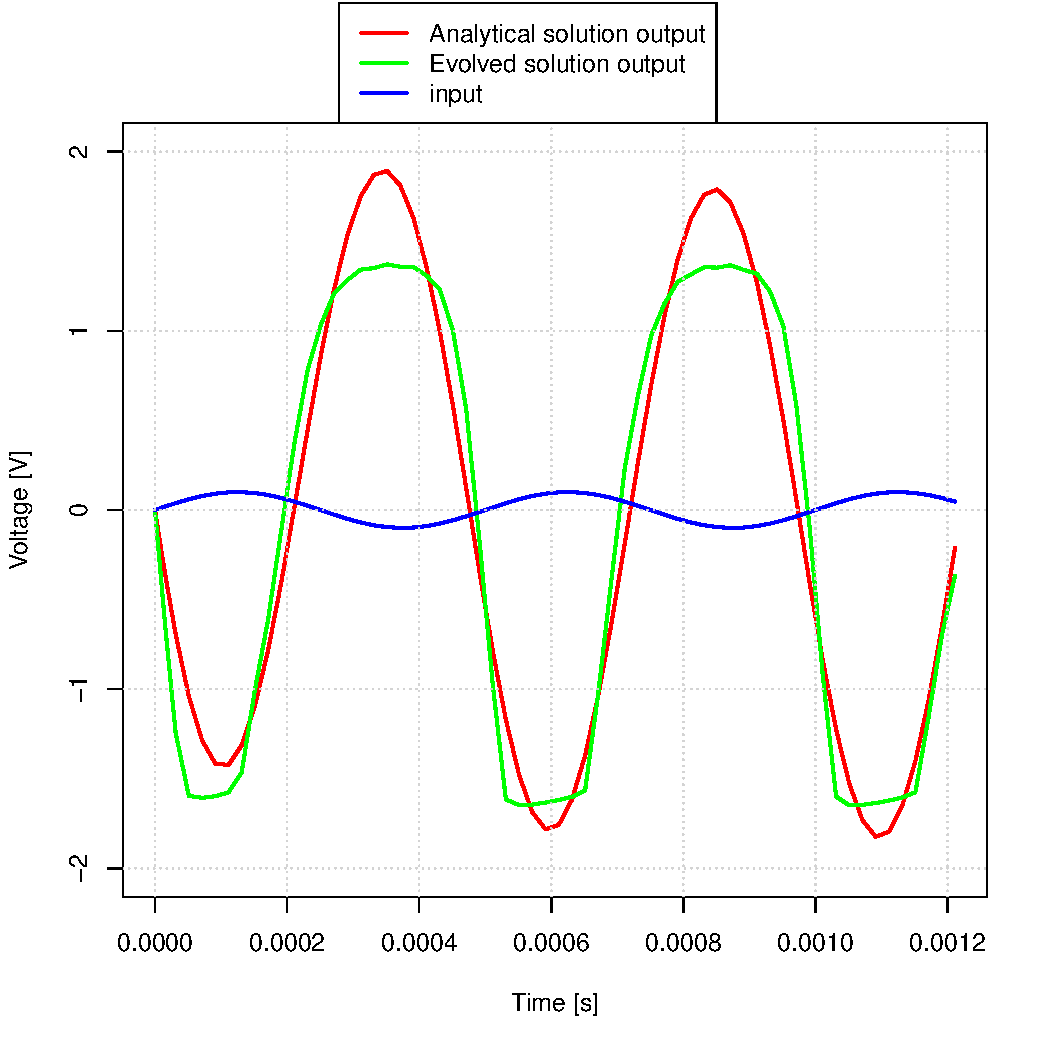
\includegraphics[scale=0.45]{evolutionCourse/graph28} \end{frame}
\begin{frame}{Evolution example} \centering 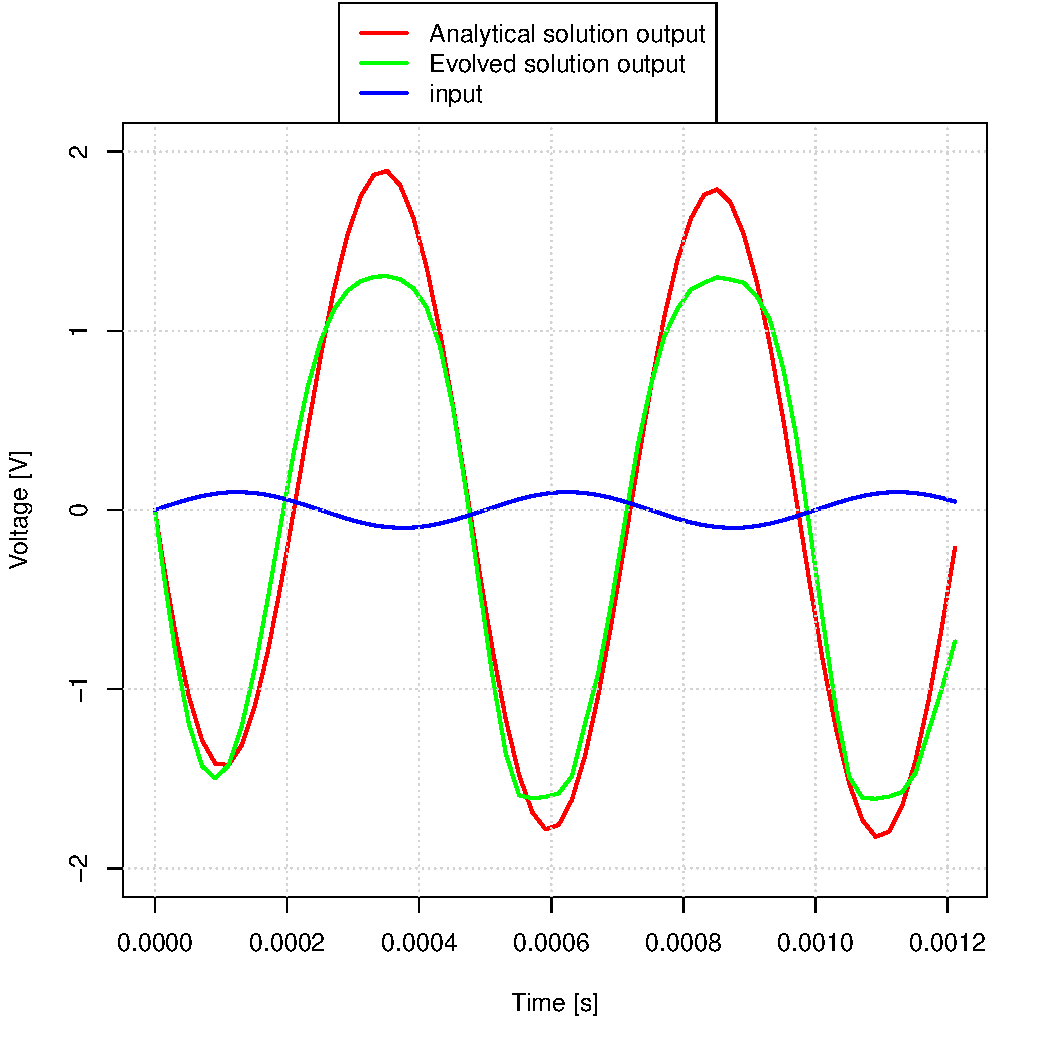
\includegraphics[scale=0.45]{evolutionCourse/graph29} \end{frame}
\begin{frame}{Evolution example} \centering 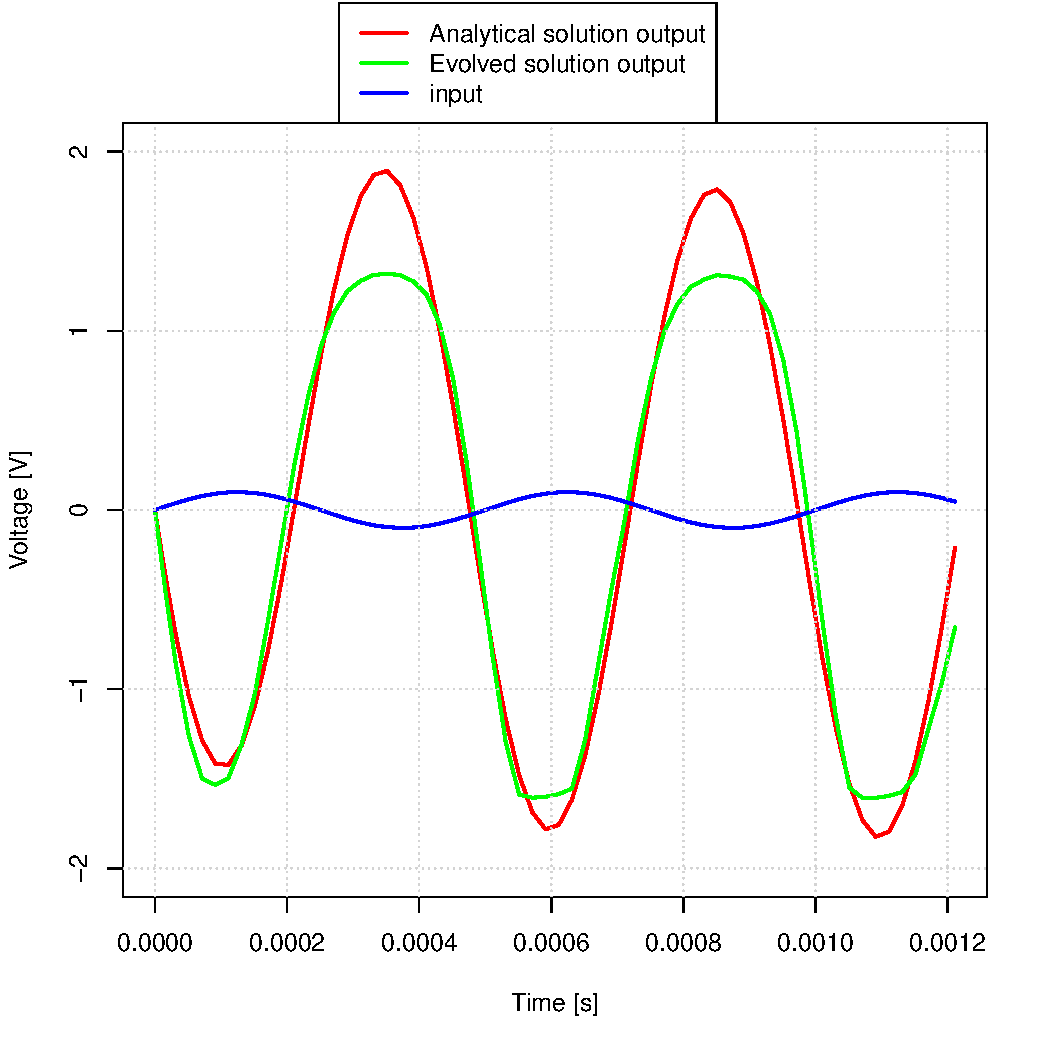
\includegraphics[scale=0.45]{evolutionCourse/graph30} \end{frame}
\begin{frame}{Evolution example} \centering 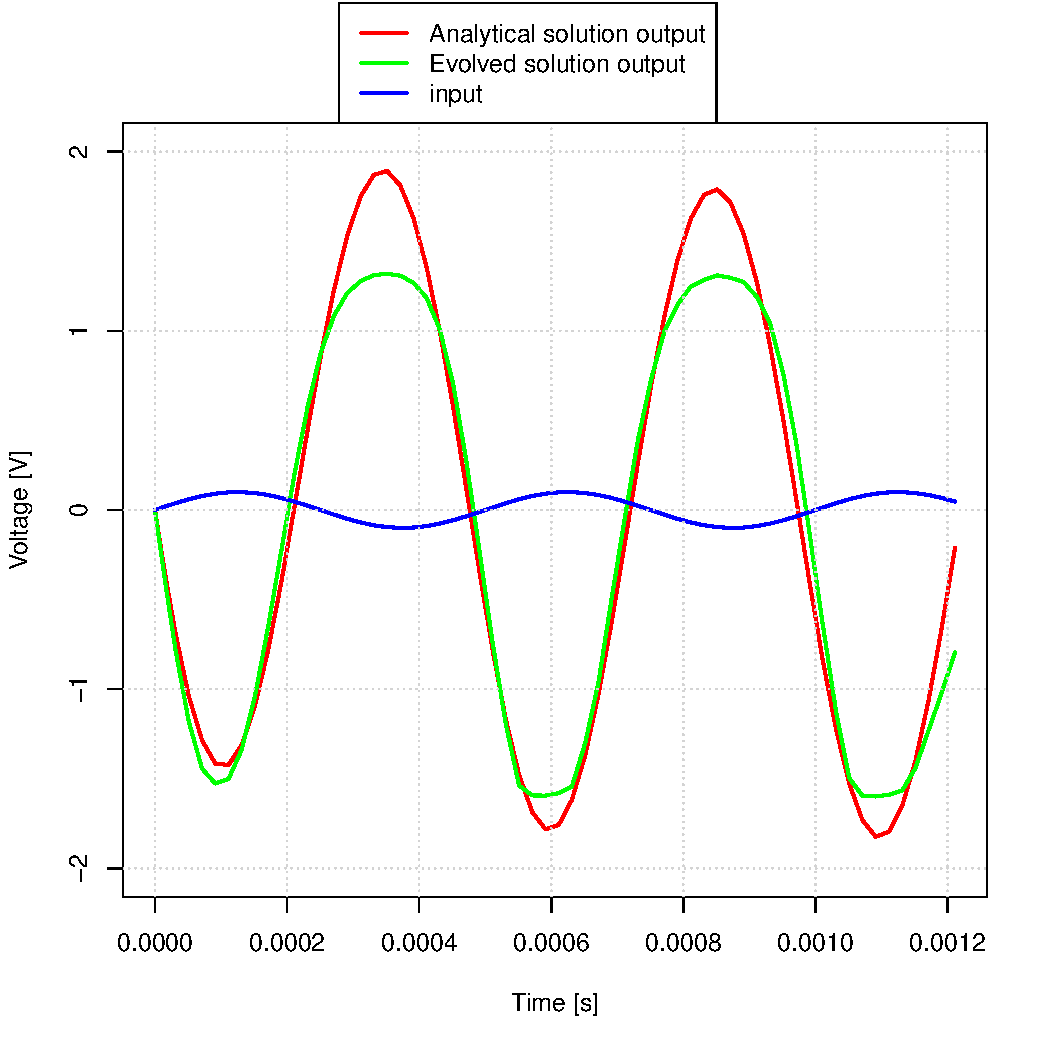
\includegraphics[scale=0.45]{evolutionCourse/graph31} \end{frame}
\begin{frame}{Evolution example} \centering 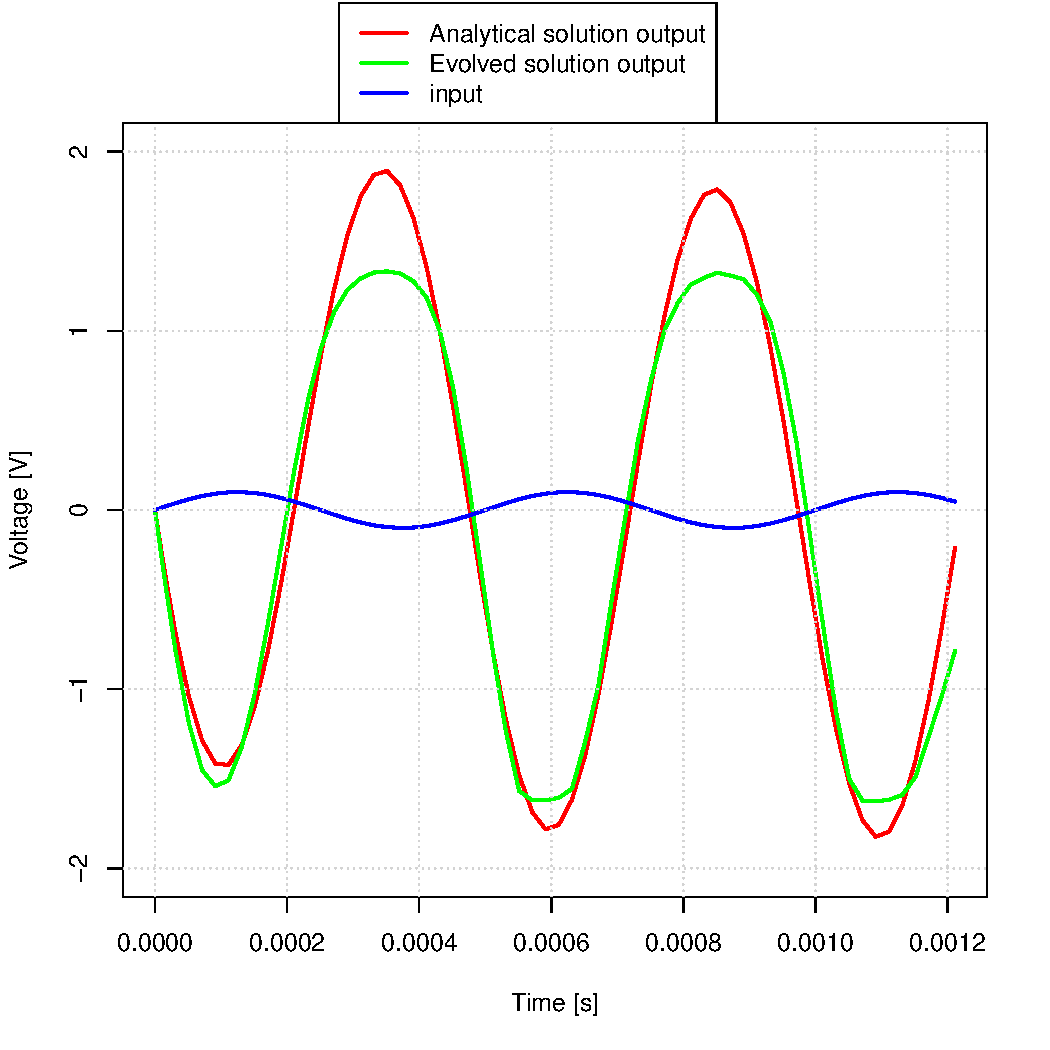
\includegraphics[scale=0.45]{evolutionCourse/graph32} \end{frame}
\begin{frame}{Evolution example} \centering 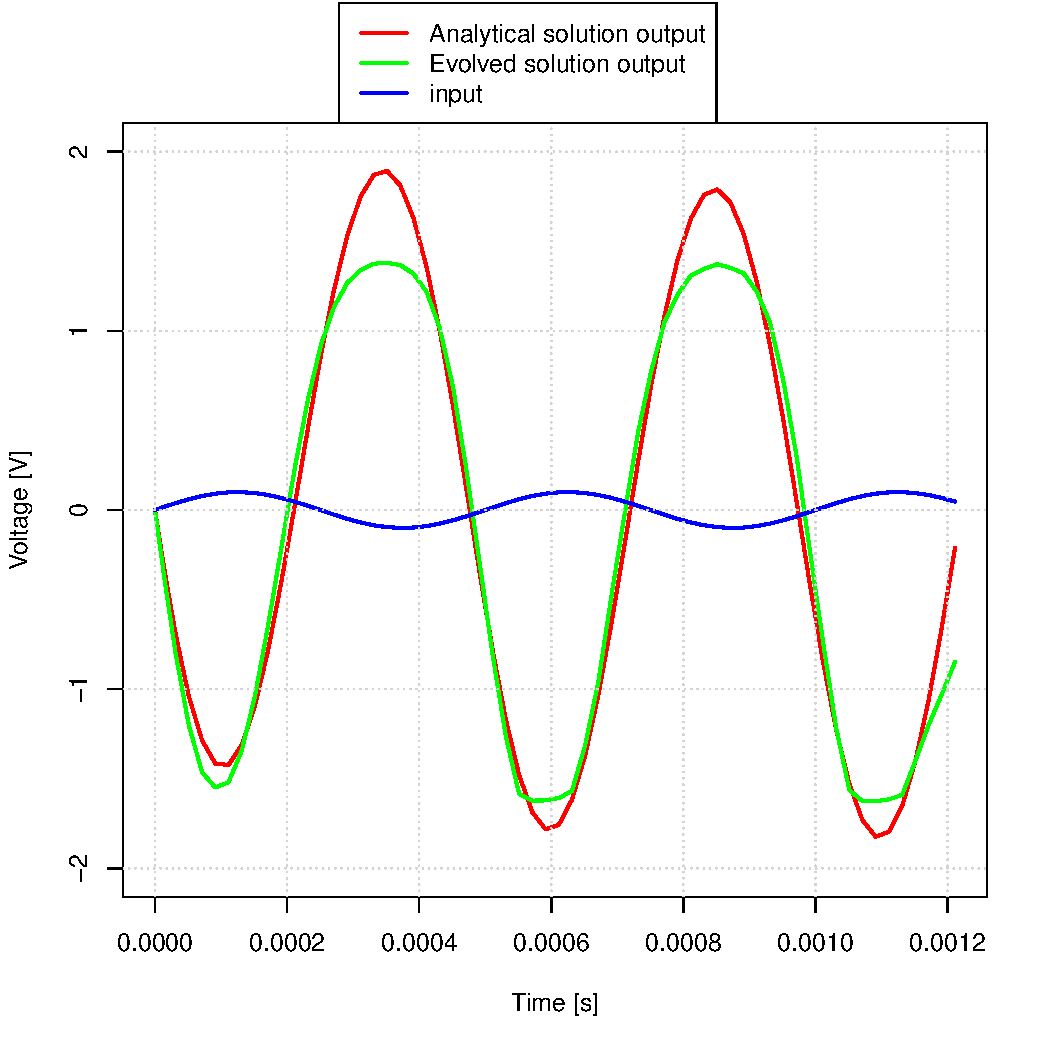
\includegraphics[scale=0.45]{evolutionCourse/graph33} \end{frame}
\begin{frame}{Evolution example} \centering 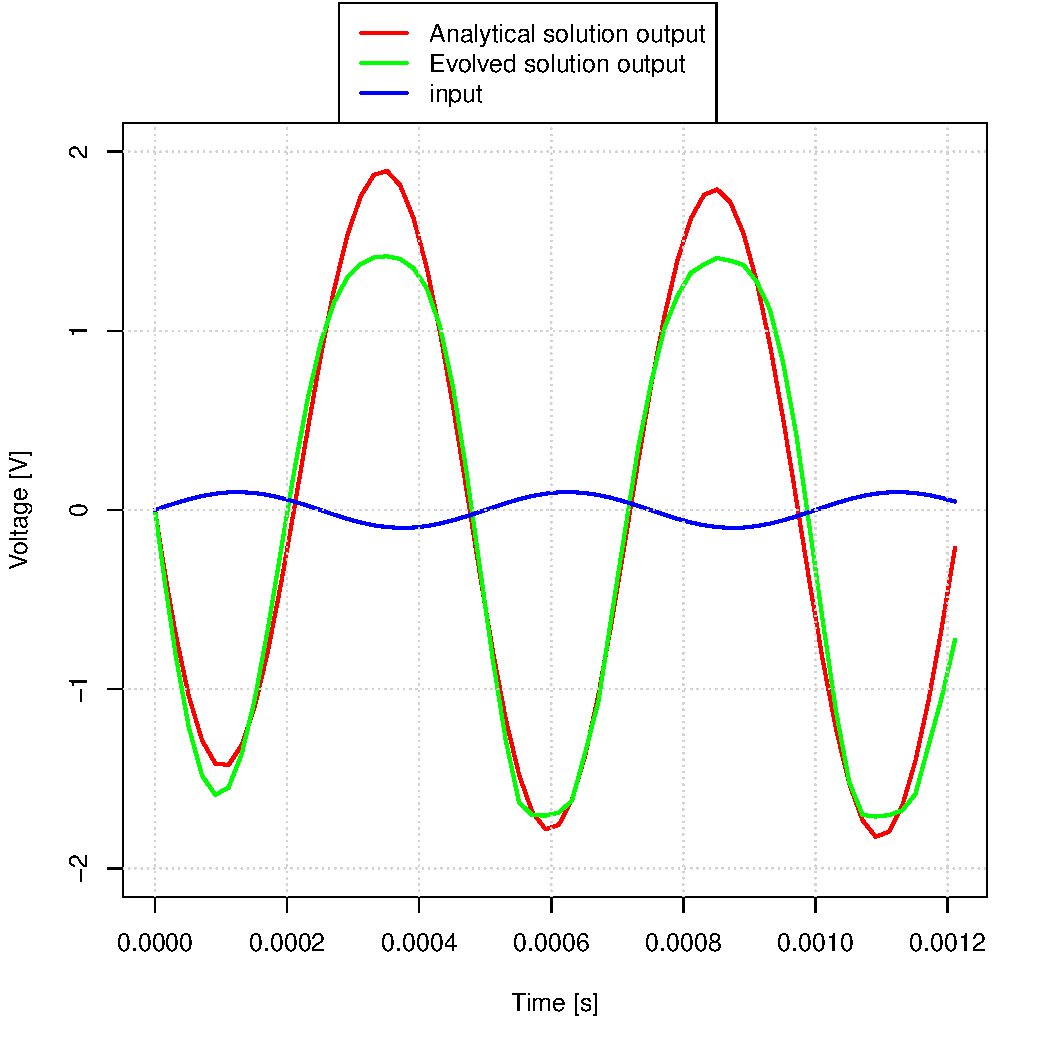
\includegraphics[scale=0.45]{evolutionCourse/graph34} \end{frame}
\begin{frame}{Evolution example} \centering 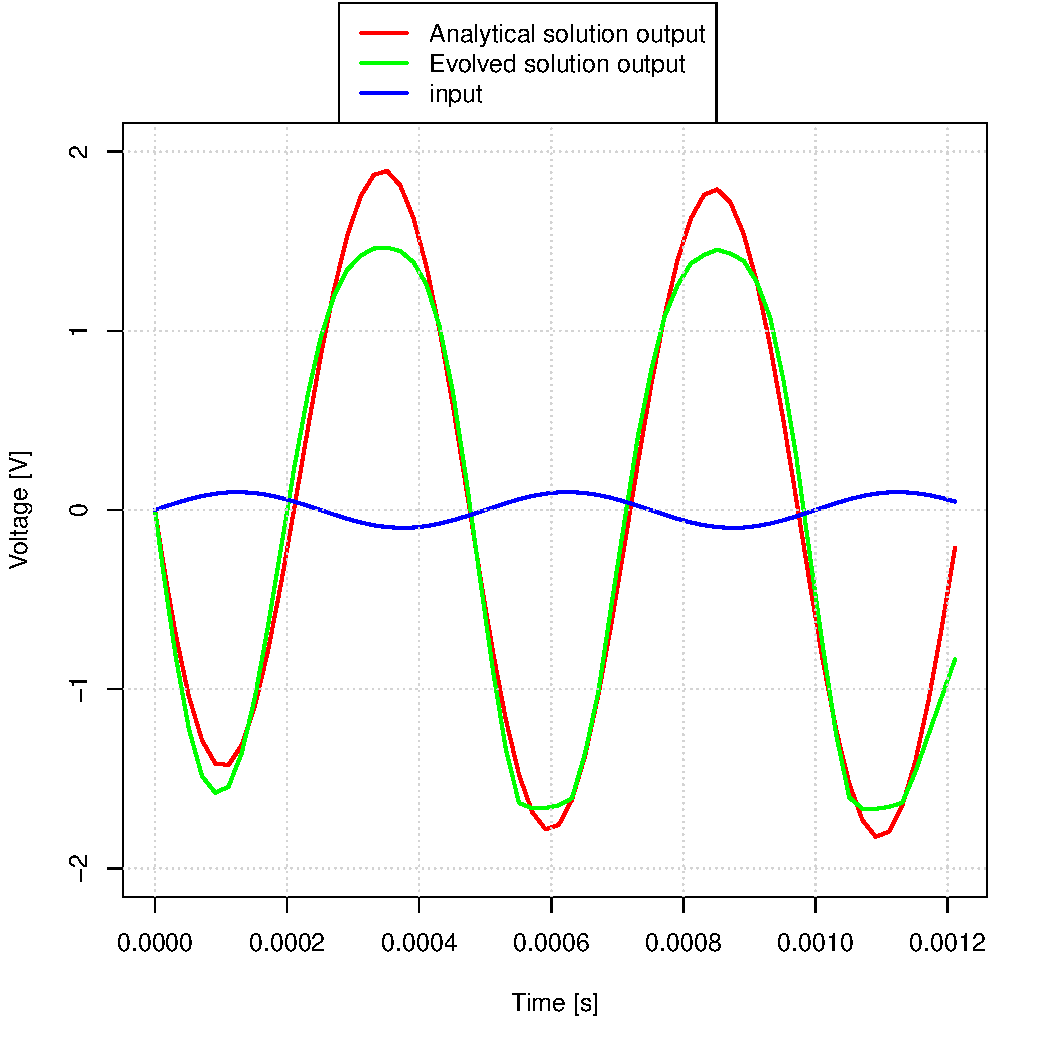
\includegraphics[scale=0.45]{evolutionCourse/graph35} \end{frame}
\begin{frame}{Evolution example} \centering 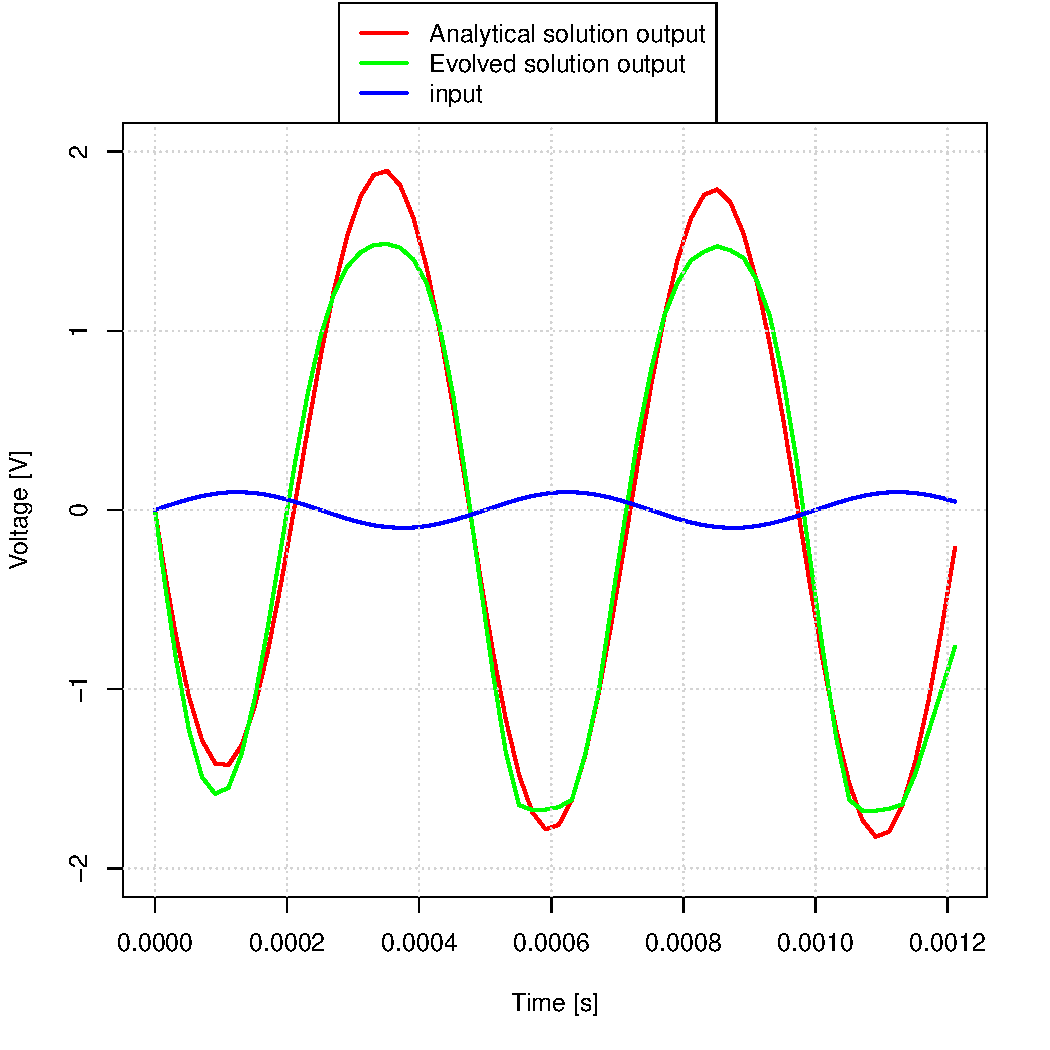
\includegraphics[scale=0.45]{evolutionCourse/graph36} \end{frame}
\begin{frame}{Evolution example} \centering 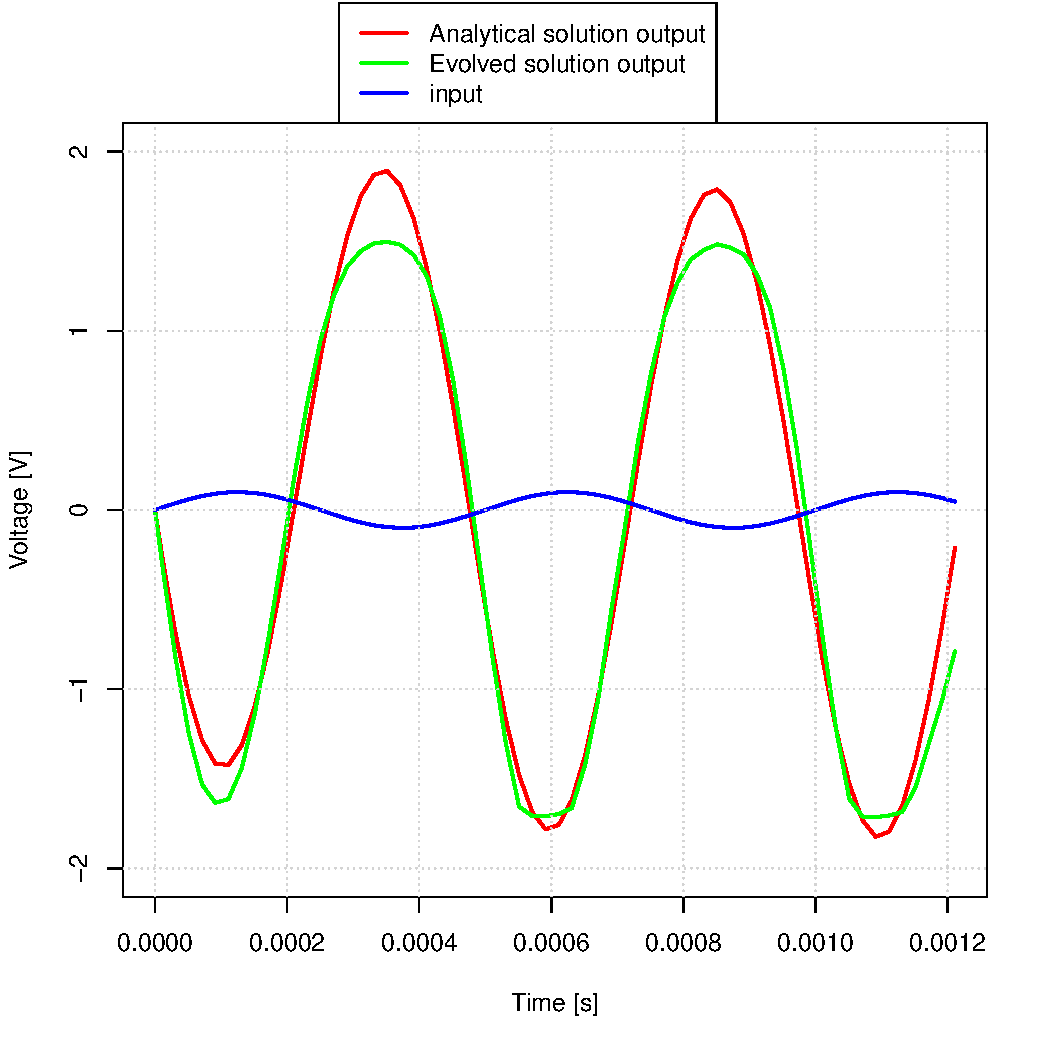
\includegraphics[scale=0.45]{evolutionCourse/graph37} \end{frame}
\begin{frame}{Evolution example} \centering 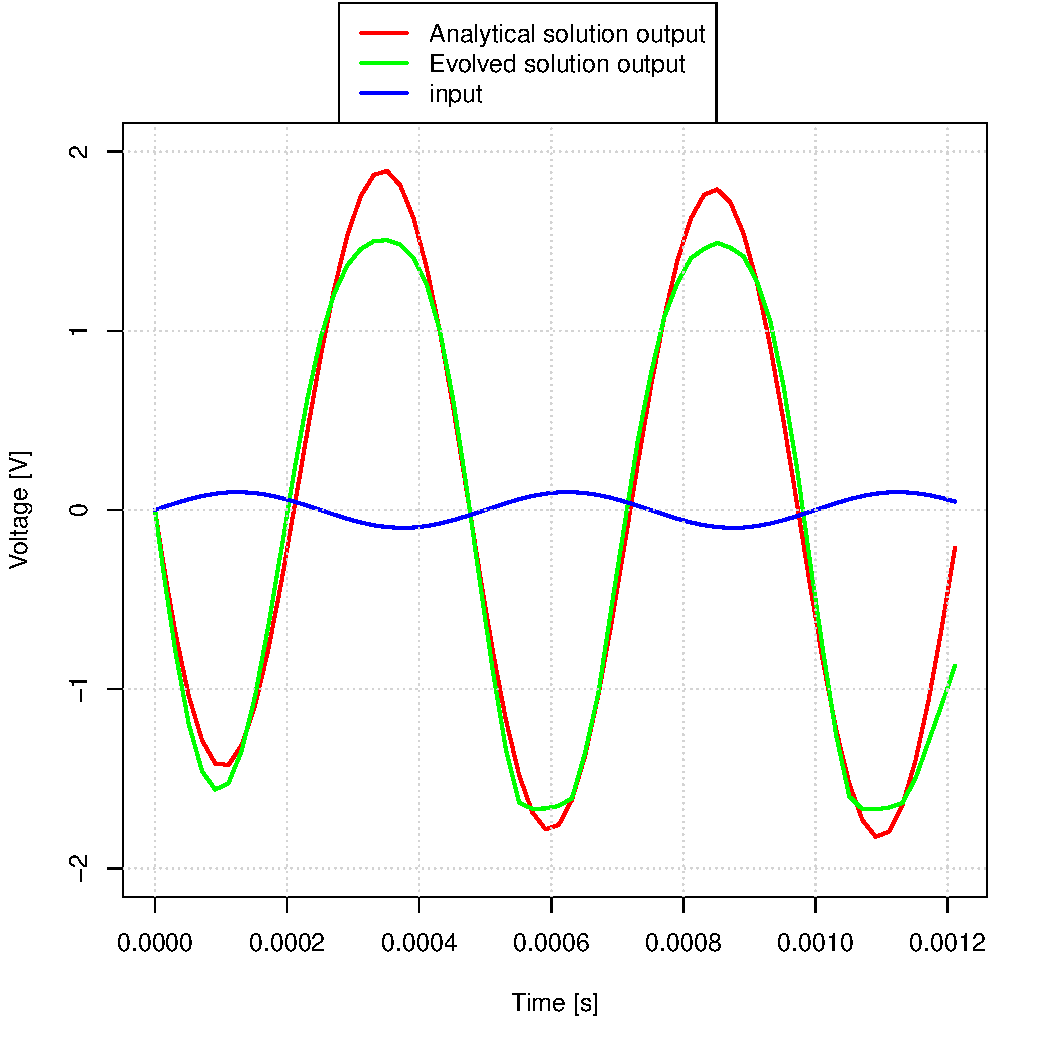
\includegraphics[scale=0.45]{evolutionCourse/graph38} \end{frame}
\begin{frame}{Evolution example} \centering 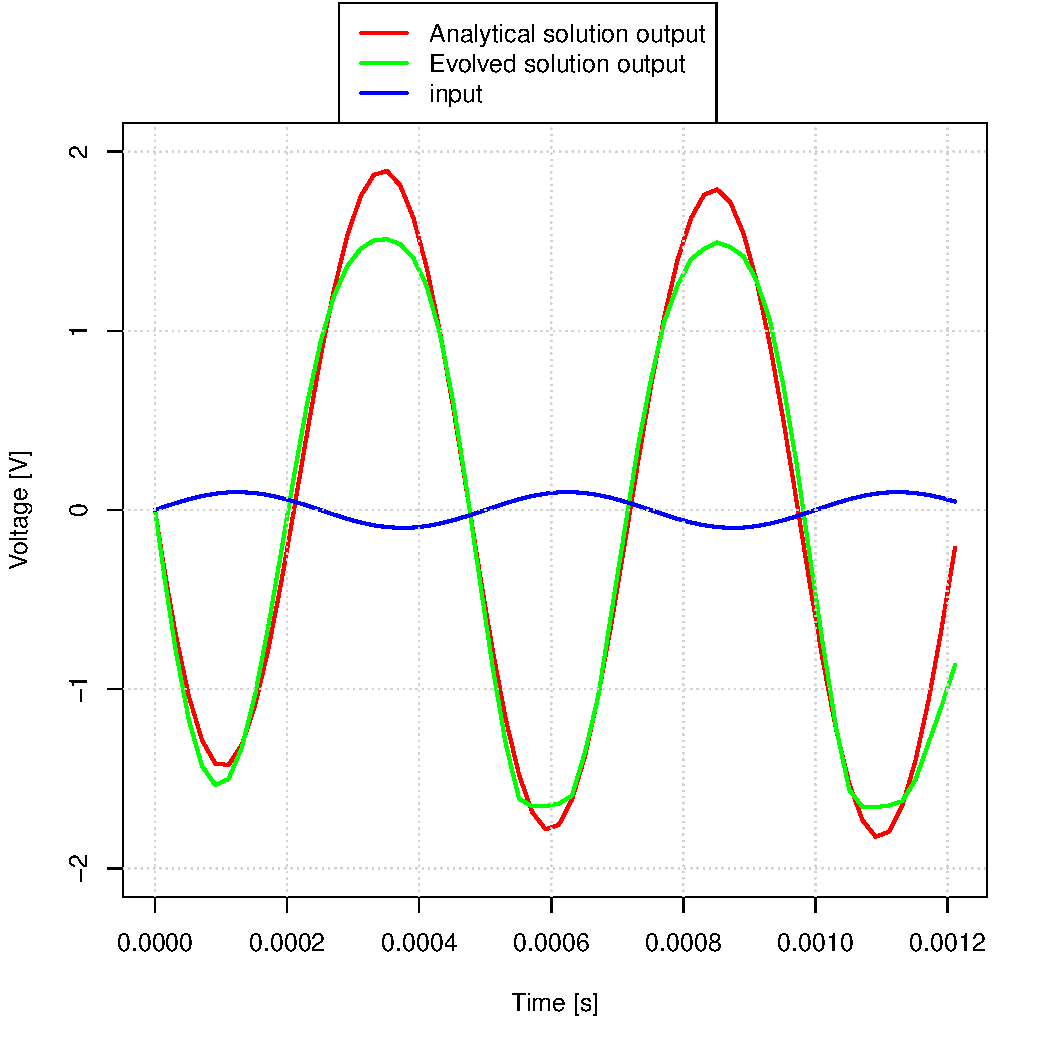
\includegraphics[scale=0.45]{evolutionCourse/graph39} \end{frame}
\begin{frame}{Evolution example} \centering 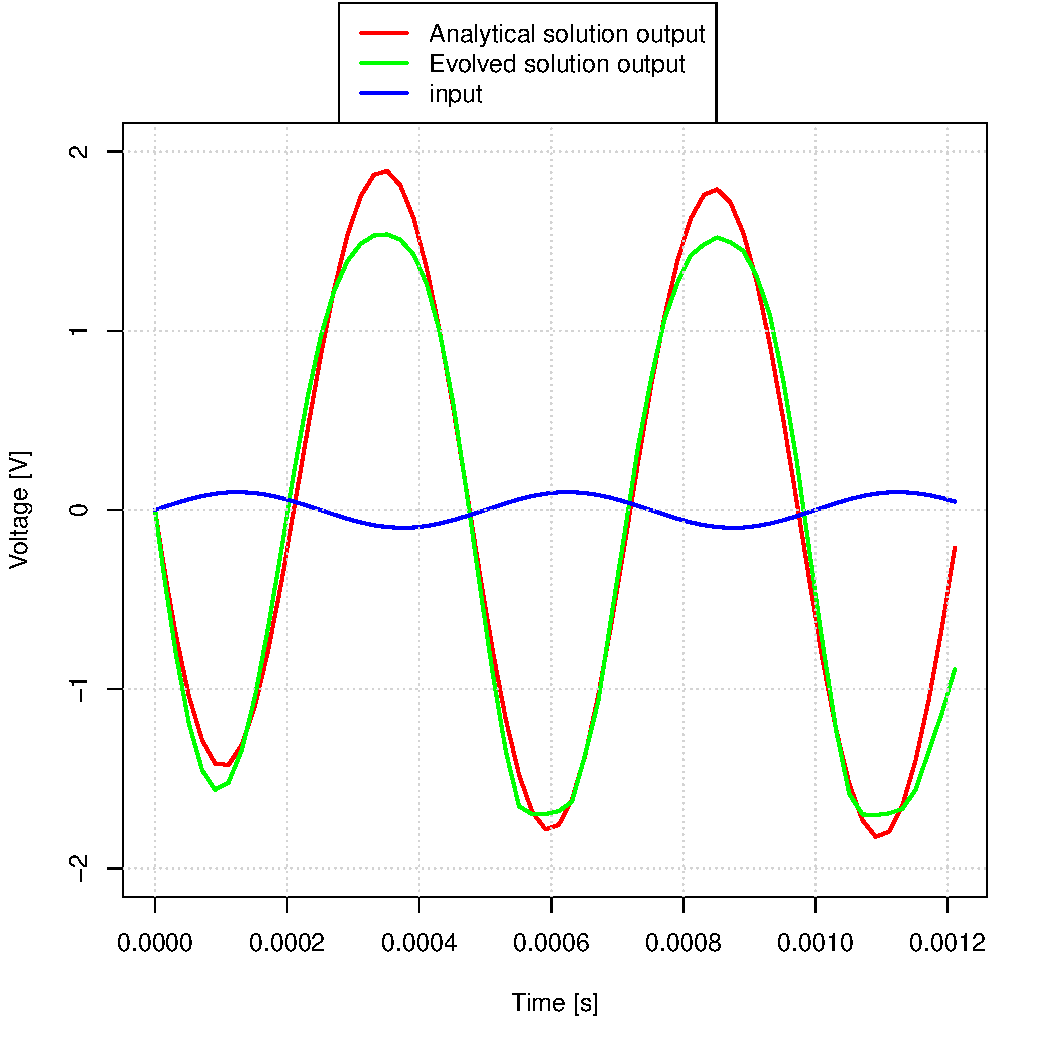
\includegraphics[scale=0.45]{evolutionCourse/graph40} \end{frame}
\begin{frame}{Evolution example} \centering 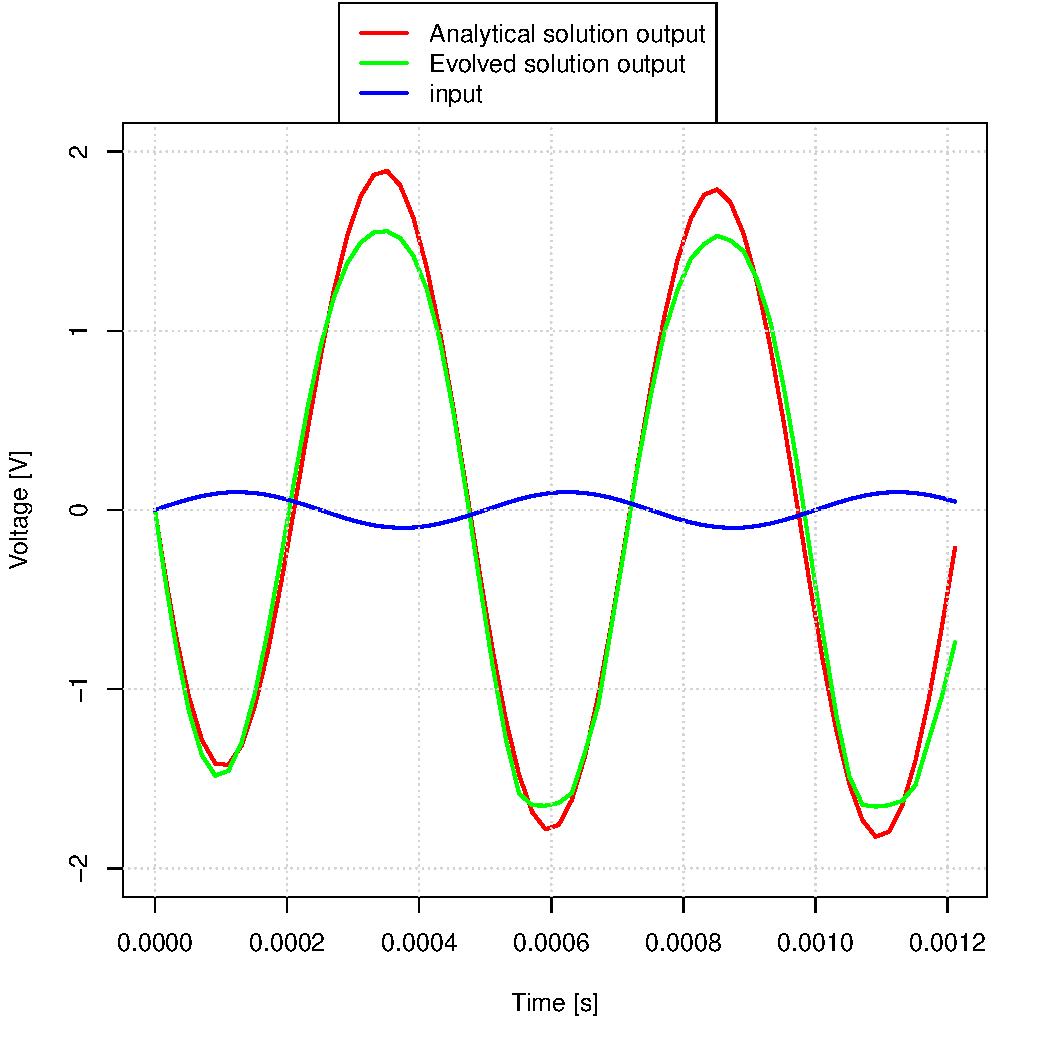
\includegraphics[scale=0.45]{evolutionCourse/graph41} \end{frame}
\begin{frame}{Evolution example} \centering 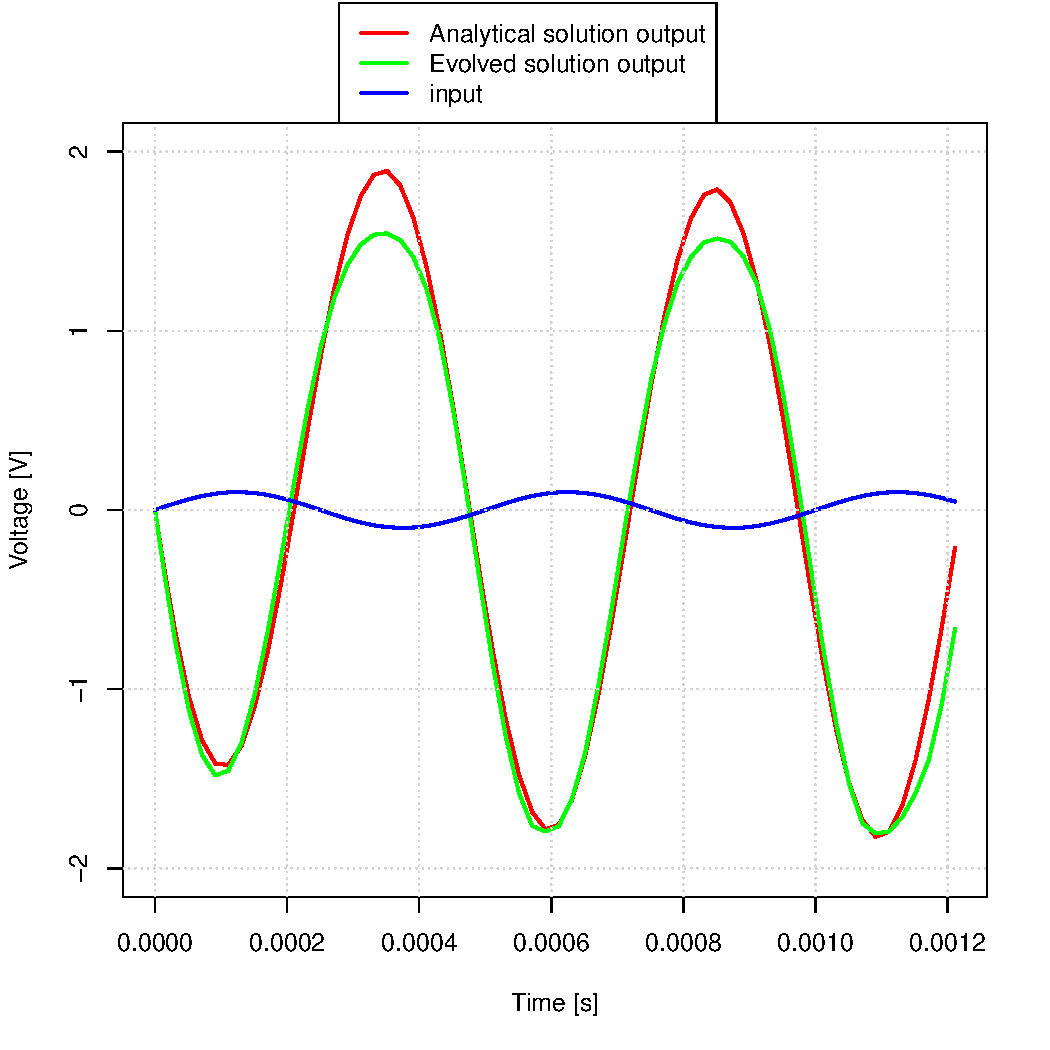
\includegraphics[scale=0.45]{evolutionCourse/graph42} \end{frame}
\begin{frame}{Evolution example} \centering 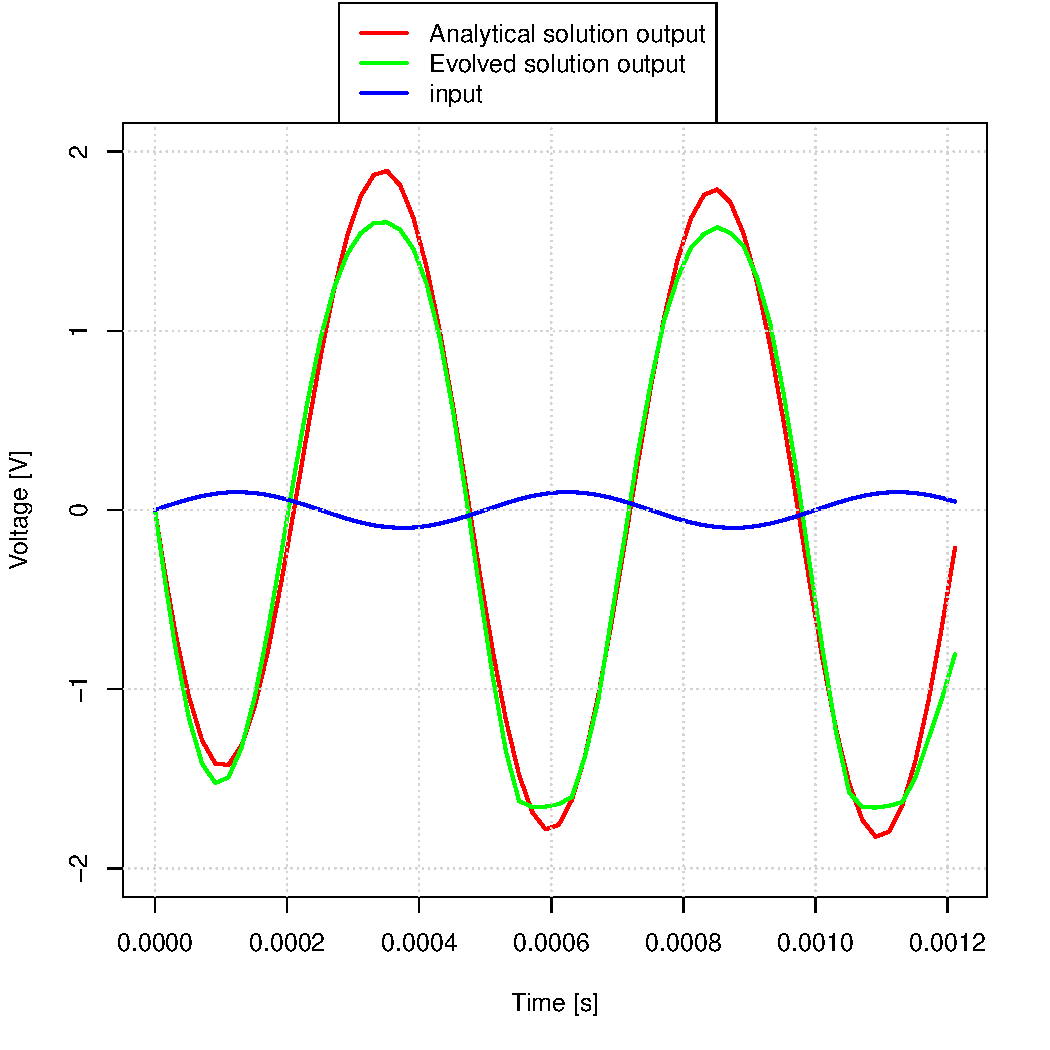
\includegraphics[scale=0.45]{evolutionCourse/graph43} \end{frame}
\begin{frame}{Evolution example} \centering \includegraphics[scale=0.45]{evolutionCourse/graph44} \end{frame}
\begin{frame}{Evolution example} \centering \includegraphics[scale=0.45]{evolutionCourse/graph45} \end{frame}
\begin{frame}{Evolution example} \centering \includegraphics[scale=0.45]{evolutionCourse/graph46} \end{frame}
\begin{frame}{Evolution example} \centering \includegraphics[scale=0.45]{evolutionCourse/graph47} \end{frame}
\begin{frame}{Evolution example} \centering \includegraphics[scale=0.45]{evolutionCourse/graph48} \end{frame}
\begin{frame}{Evolution example} \centering \includegraphics[scale=0.45]{evolutionCourse/graph49} \end{frame}
\begin{frame}{Evolution example} \centering \includegraphics[scale=0.45]{evolutionCourse/graph50} \end{frame}


\bluepage{Thank you.}

\begin{frame}{Experiments}
    \centering
    \includegraphics[scale=0.33]{ce-amplifier-simplified}

     \[
        \vec{x} = ((x_1,...,x_n), \sigma_1,...,\sigma_n)
     \]
\end{frame}

\begin{frame}{Experiments}
    \centerline{\includegraphics[scale=0.45]{evolution-course}}
\end{frame}

\begin{frame}{Experiments}
\begin{table}[H]
\centering
\begin{adjustbox}{max width=\textwidth}
\begin{tabular}{@{}ccccccccc@{}}
\toprule
    &       &           & \multicolumn{3}{c}{($\mu$, $\lambda$)-ES} & \multicolumn{3}{c}{($\mu + \lambda$)-ES} \\
   \cmidrule(lr){4-6} \cmidrule(lr){7-9}
    & $\mu$ & $\lambda$ & best match & ideal sin & max. ampl.       & best match & ideal sin  & max. ampl.     \\
   \midrule
1.  & 1     & 1         & N/A        & N/A       & N/A              & 21.82      & 99.00      & 2.90           \\
2.  & 1     & 5         & 20.82      & 113.75    & 1.98             & 13.44      & 57.91      & 2.69           \\
3.  & 1     & 10        & 18.84      & 76.81     & 1.40             & 24.70      & 75.01      & 2.84           \\
4.  & 1     & 15        & 18.43      & 128.75    & 2.26             & 19.52      & 34.11      & 1.02           \\
5.  & 5     & 5         & \textbf{49.62}      & \textbf{169.02}    & \textbf{36.50}            & 9.81       & 56.61      & 3.18           \\
6.  & 5     & 25        & 7.28       & 55.00     & 3.12             & 12.12      & 34.88      & 2.72           \\
7.  & 5     & 50        & 16.18      & 64.22     & 3.21             & 9.75       & 43.73      & 3.57           \\
8.  & 5     & 75        & 3.70       & 58.82     & 3.10             & 4.20       & 38.84      & 3.52           \\
9.  & 10    & 10        & \textbf{49.41}      & \textbf{154.66}    & \textbf{26.40}            & 8.94       & 53.77      & 3.18           \\
10. & 10    & 50        & 9.09       & 60.93     & 2.68             & 7.02       & 45.04      & 3.58           \\
11. & 10    & 100       & 6.97       & 38.02     & 3.16             & 4.91       & 26.06      & 3.10           \\
12. & 10    & 150       & 8.06       & 25.54     & 3.10             & 2.52       & 23.07      & 3.07           \\
13. & 15    & 15        & \textbf{44.48}      & \textbf{165.76}    & \textbf{34.99}            & 2.54       & 47.69      & 3.18           \\
14. & 15    & 75        & 4.64       & 56.18     & 2.25             & 4.96       & 51.74      & 3.56           \\
15. & 15    & 150       & 6.63       & 47.32     & 3.52             & 6.36       & 12.19      & 1.60           \\
16. & 15    & 225       & 7.56       & 31.17     & 2.65             & 0.70       & 19.31      & 1.08           \\
    \bottomrule
\end{tabular}
\end{adjustbox}
\end{table}
\end{frame}

\end{document}
